\documentclass{beamer}

%\usepackage[table]{xcolor}
\mode<presentation> {
  \usetheme{Boadilla}
%  \usetheme{Pittsburgh}
%\usefonttheme[2]{sans}
\renewcommand{\familydefault}{cmss}
%\usepackage{lmodern}
%\usepackage[T1]{fontenc}
%\usepackage{palatino}
%\usepackage{cmbright}
  \setbeamercovered{transparent}
\useinnertheme{rectangles}
}
%\usepackage{normalem}{ulem}
%\usepackage{colortbl, textcomp}
\setbeamercolor{normal text}{fg=black}
\setbeamercolor{structure}{fg= black}
\definecolor{trial}{cmyk}{1,0,0, 0}
\definecolor{trial2}{cmyk}{0.00,0,1, 0}
\definecolor{darkgreen}{rgb}{0,.4, 0.1}
\usepackage{array}
\beamertemplatesolidbackgroundcolor{white}  \setbeamercolor{alerted
text}{fg=red}

\setbeamertemplate{caption}[numbered]\newcounter{mylastframe}

%\usepackage{color}
\usepackage{tikz}
\usetikzlibrary{arrows}
\usepackage{colortbl}
%\usepackage[usenames, dvipsnames]{color}
%\setbeamertemplate{caption}[numbered]\newcounter{mylastframe}c
%\newcolumntype{Y}{\columncolor[cmyk]{0, 0, 1, 0}\raggedright}
%\newcolumntype{C}{\columncolor[cmyk]{1, 0, 0, 0}\raggedright}
%\newcolumntype{G}{\columncolor[rgb]{0, 1, 0}\raggedright}
%\newcolumntype{R}{\columncolor[rgb]{1, 0, 0}\raggedright}

%\begin{beamerboxesrounded}[upper=uppercol,lower=lowercol,shadow=true]{Block}
%$A = B$.
%\end{beamerboxesrounded}}
\renewcommand{\familydefault}{cmss}
%\usepackage[all]{xy}

\usepackage{tikz}
\usepackage{lipsum}

 \newenvironment{changemargin}[3]{%
 \begin{list}{}{%
 \setlength{\topsep}{0pt}%
 \setlength{\leftmargin}{#1}%
 \setlength{\rightmargin}{#2}%
 \setlength{\topmargin}{#3}%
 \setlength{\listparindent}{\parindent}%
 \setlength{\itemindent}{\parindent}%
 \setlength{\parsep}{\parskip}%
 }%
\item[]}{\end{list}}
\usetikzlibrary{arrows}
%\usepackage{palatino}
%\usepackage{eulervm}
\usecolortheme{lily}
\newtheorem{com}{Comment}
\newtheorem{lem} {Lemma}
\newtheorem{prop}{Proposition}
\newtheorem{thm}{Theorem}
\newtheorem{defn}{Definition}
\newtheorem{cor}{Corollary}
\newtheorem{obs}{Observation}
 \numberwithin{equation}{section}
%\usepackage[latin1]{inputenc}
\title[Text as Data] % (optional, nur bei langen Titeln nötig)
{Text as Data}

\author{Justin Grimmer}
\institute[University of Chicago]{Associate Professor\\Department of Political Science \\University of Chicago}
\vspace{0.3in}


\date{November 6th, 2017}%[Big Data Workshop]
%\date{\today}



\begin{document}
\begin{frame}
\titlepage
\end{frame}



\begin{frame}
\frametitle{Discovery and Measurement}

What is the research process? (Grimmer, Roberts, and Stewart 2017)

\begin{itemize}
  \item[1)] \alert{Discovery}: a hypothesis or view of the world
  \item[2)] \alert{Measurement} according to some organization
  \item[3)] \alert{Causal Inference}: effect of some intervention
\end{itemize}

Text as data methods assist at each stage of research process

\end{frame}




\begin{frame}

\huge

Text as Data Methods for Discovery \pause

\invisible<1>{Goal: Automatically Discover Organization (Similar Groups)}



\end{frame}




\begin{frame}
\frametitle{Texts and Geometry}

Consider a document-term matrix

\begin{eqnarray}
\boldsymbol{X} & = & \begin{pmatrix}
1 & 2 & 0 & \hdots & 0 \\
0 & 0 & 3 & \hdots & 0 \\
\vdots & \vdots & \vdots & \ddots & \vdots \\
1 & 0 & 0 & \hdots & 3 \\
\end{pmatrix}\nonumber
\end{eqnarray}


\pause \invisible<1>{Suppose documents live in a \alert{space}}\pause\invisible<1-2>{ $\leadsto$ rich set of results from linear algebra} \pause
\begin{itemize}
\invisible<1-3>{\item[-] Provides a \alert{geometry}}\pause\invisible<1-4>{$\leadsto$ modify with word weighting} \pause
\invisible<1-5>{\item[-] Natural notions of \alert{distance}} \pause
\invisible<1-6>{\item[-] Building block for clustering, supervised learning, and scaling}
\end{itemize}



\end{frame}



\begin{frame}
\frametitle{Texts in Space}
\pause
\begin{eqnarray}
\invisible<1>{\text{Doc1} & = & (1, 1, 3, \hdots, 5) \nonumber \\ } \pause
\invisible<1-2>{\text{Doc2} & = & (2, 0, 0, \hdots, 1) \nonumber \\} \pause
\invisible<1-3>{\textbf{Doc1}, \textbf{Doc2} & \in & \Re^{J} \nonumber } \pause
\end{eqnarray}



\invisible<1-4>{\alert{Inner Product} between documents: } \pause
\begin{eqnarray}
\invisible<1-5>{\textbf{Doc1} \cdot \textbf{Doc2}  &  = &  (1, 1, 3, \hdots, 5)^{'} (2, 0, 0, \hdots, 1) \nonumber \\} \pause
\invisible<1-6>{  & = &  1 \times 2 + 1 \times 0 + 3 \times 0 + \hdots + 5 \times 1  \nonumber \\} \pause
\invisible<1-7>{   & = & 7 \nonumber}
   \end{eqnarray}

\end{frame}


\begin{frame}
\frametitle{Vector Length}

\begin{columns}[]

\column{0.6\textwidth}
\only<1>{\scalebox{0.5}{\includegraphics{Length1.pdf}}}
\only<2>{\scalebox{0.5}{\includegraphics{Length2.pdf}}}
\only<3>{\scalebox{0.5}{\includegraphics{Length3.pdf}}}
\only<4-5>{\scalebox{0.5}{\includegraphics{Length4.pdf}}}

\column{0.4\textwidth}
\begin{itemize}
\invisible<1>{\item[-] \alert{Pythagorean Theorem}: Side with length $a$}
\invisible<1-2>{\item[-] Side with length $b$ and right triangle}
\invisible<1-3>{\item[-] $c = \sqrt{ a^2 + b^2} $ }
\invisible<1-4>{\item[-] \alert{This is generally true} }
\end{itemize}

\end{columns}

\pause \pause \pause \pause
\end{frame}




\begin{frame}
\frametitle{Vector (Euclidean) Length}

\begin{defn} Suppose $\boldsymbol{v} \in \Re^{J}$. Then, we will define its \alert{length} as
\begin{eqnarray}
||\boldsymbol{v}|| & = & (\boldsymbol{v} \cdot \boldsymbol{v} )^{1/2} \nonumber \\
               & = & (v_{1}^2 + v_{2}^{2} + v_{3}^{2} + \hdots + v_{J}^{2} )^{1/2} \nonumber
\end{eqnarray}
\end{defn}


\end{frame}


\begin{frame}
\frametitle{Measures of Dissimilarity}

Initial guess$\leadsto$ \alert{Distance metrics} \\

Properties of a metric: (distance function) $d(\cdot, \cdot)$.  Consider arbitrary documents $\boldsymbol{X}_{i}$, $\boldsymbol{X}_{j}$, $\boldsymbol{X}_{k}$ \pause
\begin{itemize}
\invisible<1>{\item[1)] $d(\boldsymbol{X}_{i}, \boldsymbol{X}_{j}) \geq 0$} \pause
\invisible<1-2>{\item[2)] $d(\boldsymbol{X}_{i}, \boldsymbol{X}_{j} ) = 0 $ if and only if $\boldsymbol{X}_{i} = \boldsymbol{X}_{j}$} \pause
\invisible<1-3>{\item[3)] $d(\boldsymbol{X}_{i}, \boldsymbol{X}_{j} ) = d(\boldsymbol{X}_{j}, \boldsymbol{X}_{i} )$} \pause
\invisible<1-4>{\item[4)] $d(\boldsymbol{X}_{i}, \boldsymbol{X}_{k}) \leq d(\boldsymbol{X}_{i}, \boldsymbol{X}_{j})  + d(\boldsymbol{X}_{j}, \boldsymbol{X}_{k})$} \pause
\end{itemize}

\vspace{0.5in}

\invisible<1-5>{Explore \alert{distance} functions to compare documents}$\leadsto$\pause\invisible<1-6>{Do we want additional assumptions/properties?}

\end{frame}




\begin{frame}
\frametitle{Measuring the Distance Between Documents}

\alert{Euclidean Distance}


\begin{center}
\only<1>{\scalebox{0.5}{\includegraphics{Doc1.pdf}}}
\only<2>{\scalebox{0.5}{\includegraphics{Doc2.pdf}}}
\only<3>{\scalebox{0.5}{\includegraphics{Doc3.pdf}}}
\end{center}



\end{frame}


\begin{frame}
\frametitle{Measuring the Distance Between Documents}

\begin{defn}
The Euclidean distance between documents $\boldsymbol{X}_{i}$ and $\boldsymbol{X}_{j}$ as

\begin{eqnarray}
||\boldsymbol{X}_{i} - \boldsymbol{X}_{j}||  & =  & \sqrt{\sum_{m=1}^{J} \left(x_{im} -  x_{jm} \right)^2} \nonumber
\end{eqnarray}

\end{defn}

\pause
\invisible<1>{Suppose $\boldsymbol{X}_{i} = (1, 4)$ and $\boldsymbol{X}_{j} = (2, 1)$.  The distance between the documents is:
\begin{eqnarray}
||(1, 4) - (2,1) || & = & \sqrt{ (1 -2 )^2 + (4 - 1)^2 } \nonumber\\
   & = & \sqrt{10}  \nonumber
\end{eqnarray}
}

\end{frame}



\begin{frame}
\frametitle{Measuring Similarity (and removing document length)}



\pause

\invisible<1>{What properties should similarity measure have?} \pause
\begin{itemize}
\invisible<1-2>{\item[-] Maximum: document with itself} \pause
\invisible<1-3>{\item[-] Minimum: documents have no words in common (\alert{orthogonal} ) } \pause
\invisible<1-4>{\item[-] Increasing when \alert{more} of same words used } \pause
\invisible<1-5>{\item[-] \alert{?} $s(a, b)  = s(b,a)$.  }  \pause
\end{itemize}

\invisible<1-6>{How should additional words be treated?}


\end{frame}



\begin{frame}
\frametitle{Measuring Similarity}

\begin{center}
\scalebox{0.35}{\includegraphics{Fig1.pdf}}
\end{center}


Measure 1: Inner product \pause  \\
\begin{eqnarray}
\invisible<1>{(2, 1)^{'} \cdot (1, 4) & = & 6 }   \nonumber
\end{eqnarray}



\end{frame}



\begin{frame}

\begin{center}
\only<1-3>{\scalebox{0.35}{\includegraphics{Fig2.pdf}}}
\only<4>{\scalebox{0.35}{\includegraphics{Fig3.pdf}}}
\end{center}



\invisible<1>{\alert{Problem}(?): length dependent }
\begin{eqnarray}
\invisible<1-2>{(4,2)^{'} (1,4) & = & 12 } \nonumber \\
\invisible<1-3>{a \cdot b & = & ||a|| \times ||b|| \times \cos \theta \nonumber }
\end{eqnarray}

\pause \pause \pause



\end{frame}



\begin{frame}
\frametitle{Cosine Similarity}


\begin{center}
\only<7->{\scalebox{0.35}{\includegraphics{Fig4.pdf}}}
\end{center}


\only<7->{
$\cos \theta$: removes document length from similarity measure\\ \pause
\invisible<1-7>{Projects texts to unit length representation$\leadsto$ onto sphere}
}


\only<1-6>{\begin{eqnarray}
\invisible<1>{\cos \theta & = & \left(\frac{a} {||a||}\right)  \cdot \left(\frac{b} {||b||}  \right) \nonumber \\}
\invisible<1-2>{\frac{(4,2)}{||(4,2) ||} & = & (0.89, 0.45) \nonumber \\}
\invisible<1-3>{\frac{(2,1)}{||(2,1) || } & = & (0.89, 0.45) \nonumber \\}
\invisible<1-4>{\frac{(1,4)} {||(1,4)||}  & = & (0.24, 0.97) \nonumber } \\
\invisible<1-5>{(0.89, 0.45)^{'} (0.24, 0.97) & = & 0.65 \nonumber }
\end{eqnarray}
}

\pause \pause \pause \pause \pause \pause \pause

\end{frame}



\begin{frame}
\frametitle{Weighting Words}

Are all words created equal?  \pause
\begin{itemize}
\invisible<1>{\item[-] Treat all words equally} \pause
\invisible<1-2>{\item[-] \alert{Lots of noise} } \pause
\invisible<1-3>{\item[-] Reweight words} \pause
\begin{itemize}
\invisible<1-4>{\item[-] Accentuate words that are likely to be \alert{informative}} \pause
\invisible<1-5>{\item[-] Make specific assumptions about characteristics of \alert{informative} words} \pause
\end{itemize}
\end{itemize}

\invisible<1-6>{How to generate weights?} \pause
\begin{itemize}
\invisible<1-7>{\item[-] Assumptions about separating words} \pause
\invisible<1-8>{\item[-] Use \alert{training} set to identify separating words (Monroe, Ideology measurement)}
\end{itemize}



\end{frame}


\begin{frame}
\frametitle{Weighting Words: TF-IDF Weighting}

What properties do words need to separate concepts? \pause
\begin{itemize}
\invisible<1>{\item[-] Used frequently} \pause
\invisible<1-2>{\item[-] But not too frequently} \pause
\end{itemize}
\invisible<1-3>{\alert{Ex.} If all statements about OBL contain {\tt Bin Laden} than this contributes nothing to similarity/dissimilarity measures\\} \pause

\invisible<1-4>{\alert{Inverse document frequency}:} \pause
\begin{eqnarray}
\invisible<1-5>{\text{n}_{j} & = & \text{No. documents in which word $j$ occurs} \nonumber \\} \pause
\invisible<1-6>{\text{idf}_{j} & = & \log \frac{N} {n_j} \nonumber  \\ } \pause
\invisible<1-7>{\textbf{idf} & = & (\text{idf}_{1} , \text{idf}_{2}, \hdots, \text{idf}_{J} ) \nonumber }
\end{eqnarray}


\end{frame}


\begin{frame}
\frametitle{Weighting Words: TF-IDF Weighting}


Why $\log$ ? \pause
\begin{itemize}
\invisible<1>{\item[-] Maximum at $n_j$ = 1} \pause
\invisible<1-2>{\item[-] Decreases at rate $\frac{1}{n_j} \Rightarrow$ diminishing ``penalty" for more common use} \pause
\invisible<1-3>{\item[-] Other functional forms are fine, embed assumptions about penalization of common use}
\end{itemize}



\end{frame}


\begin{frame}
\frametitle{Weighting Words: TF-IDF}

\pause
\begin{eqnarray}
\invisible<1>{\textbf{X}_{i, \text{idf}}  \equiv \underbrace {\textbf{X}_{i}}_{\text{tf} } \times \textbf{idf} & = & (X_{i1} \times \text{idf}_1 , X_{i2} \times \text{idf}_2 , \hdots, X_{iJ} \times \text{idf}_J) \nonumber \\} \pause
\invisible<1-2>{\textbf{X}_{j,\text{idf}}\equiv \textbf{X}_{j} \times \textbf{idf} & = & (X_{j1} \times \text{idf}_1 , X_{j2} \times \text{idf}_2 , \hdots, X_{jJ} \times \text{idf}_J ) \nonumber} \pause
\end{eqnarray}

\invisible<1-3>{How Does This Matter For Measuring Similarity/Dissimilarity? \\} \pause

\invisible<1-4>{\alert{Inner Product} } \pause
\begin{eqnarray}
\invisible<1-5>{\textbf{X}_{i, \text{idf}} \cdot \textbf{X}_{j, \text{idf}} & = &(\textbf{X}_{i} \times \textbf{idf} )^{'} ( \textbf{X}_{j} \times \textbf{idf})  \nonumber \\} \pause
\invisible<1-6>{ & = & (\text{idf}_1^2 \times  X_{i1} \times X_{j1}) + (\text{idf}^{2}_2 \times X_{i2} \times X_{j2}) + \nonumber \\
 & &  \hdots + (\text{idf}_J^{2} \times X_{iJ} \times X_{jJ}) \nonumber }
 \end{eqnarray}


\end{frame}




\begin{frame}
\frametitle{Weighting Words: Inner Product}

Define: \pause \\
\vspace{0.25in}


\invisible<1>{$\boldsymbol{\Sigma}  = \begin{pmatrix}
                      \text{idf}_1^{2} & 0 & 0 &\hdots & 0 \\
                      0 & \text{idf}_2^{2} & 0 &\hdots &0 \\
                      \vdots & \vdots & \vdots & \ddots & \vdots \\
                      0 & 0 & 0 & \hdots & \text{idf}_J^{2}
                      \end{pmatrix} $} \pause

\vspace{0.25in}
\invisible<1-2>{If we use tf-idf for our documents, then  } \pause
\begin{eqnarray}
\invisible<1-3>{d_{2}(\boldsymbol{X}_{i}, \boldsymbol{X}_{j} ) & = & \sqrt{\sum_{m=1}^{J}(x_{im, \text{idf}} - x_{jm, \text{idf}} )^{2} } \nonumber \\
 & = & \sqrt{(\boldsymbol{X}_{i}  - \boldsymbol{X}_{j})^{'}\boldsymbol{\Sigma} (\boldsymbol{X}_{i}  - \boldsymbol{X}_{j})  } \nonumber }
\end{eqnarray}


\end{frame}


\begin{frame}
\frametitle{Final Product}

Applying some measure of distance, similarity (if symmetric) yields:

$\textbf{D} = \begin{pmatrix}
0 & d (1, 2)  & d(1, 3) & \hdots & d(1, N) \\
\alert{d(2,1)} & 0 &  d(2,3)  & \hdots & d(2, N) \\
\alert{d(3,1)} & \alert{d(3,2)} & 0 & \hdots & d(3, N ) \\
\vdots & \vdots & \vdots & \ddots & \vdots \\
\alert{d(N,1)} & \alert{d(N,2)} & \alert{d(N,3)}   & \alert{\hdots}  & 0
\end{pmatrix} $


\vspace{0.5in}

\alert{Lower Triangle} contains unique information $N(N-1)/2$


\end{frame}


\begin{frame}
\frametitle{Clustering}


\alert{Fully Automated Clustering}
\begin{itemize}
\item[1)] Distance metric$\leadsto$ when are documents close?
\item[2)] Objective function $\leadsto$ how do we summarize distances?
\item[3)] Optimization method $\leadsto$ how do we find optimal clustering?
\end{itemize}
\alert{THERE IS NO A PRIORI OPTIMAL METHOD}\\
\alert{Computer Assisted Clustering (Grimmer and King, 2011) }
\begin{itemize}
\item[-] \alert{crucial} to combine human and computer insights
\end{itemize}


\end{frame}




\begin{frame}
\frametitle{K-Means$\leadsto$ Objective Function}

$N$ documents $\boldsymbol{x}_{i} = (x_{i1}, x_{i2}, \hdots, x_{iJ})$ (normalized) \pause \\
\invisible<1>{Goal$\leadsto$ Partition documents into $K$ clusters. } \pause  \\
\invisible<1-2>{Two parameters to estimate} \pause
\begin{itemize}
\invisible<1-3>{\item[1)] $K\times J$ matrix of cluster centers $\Theta$. } \pause \\
\invisible<1-4>{Cluster $k$ has center } \pause
\begin{eqnarray}
\invisible<1-5>{\boldsymbol{\theta}_{k} & = & (\theta_{1k}, \theta_{2k}, \hdots, \theta_{Jk}) \nonumber }\pause
\end{eqnarray}
\invisible<1-6>{$\boldsymbol{\theta}_{k} = $ \alert{exemplar} for cluster $k$} \pause

\invisible<1-7>{\item[2)] $\boldsymbol{T}$ is an $N \times K$ matrix. Each row is an indicator vector.\\} \pause
\invisible<1-8>{If observation $i$ is from cluster $k$, then  } \pause
\begin{eqnarray}
\invisible<1-9>{\boldsymbol{\tau}_{i} & = & (0, 0, \hdots, 0, \underbrace{1}_{k^{th}}, 0, \hdots, 0) \nonumber }\pause
\end{eqnarray}
\invisible<1-10>{\alert{Hard Assignment}}

\end{itemize}



\end{frame}




\begin{frame}
\frametitle{K-Means$\leadsto$ Objective Function}

Assume squared euclidean distance \pause

\begin{eqnarray}
\invisible<1>{f(\boldsymbol{X},\boldsymbol{T}, \boldsymbol{\Theta}) & = & \sum_{i=1}^{N} \sum_{k=1}^{K} \overbrace{\tau_{ik}}^{\text{cluster indicator}} \underbrace{\left(\sum_{j=1}^{J} (x_{ij} - \theta_{kj})^2 \right)}_{\text{Squared Euclidean Distance}} \nonumber }\pause
\end{eqnarray}

\begin{itemize}
\invisible<1-2>{\item[-] Calculate squared euclidean distance from center} \pause
\invisible<1-3>{\item[-] \alert{Only} for the assigned cluster} \pause
\invisible<1-4>{\item[-] Two trivial solutions} \pause
\begin{itemize}
\invisible<1-5>{\item[-] If $K = N$ then $f( \boldsymbol{X}, \boldsymbol{T}, \boldsymbol{\Theta})  = 0 $ (Minimum)} \pause
\begin{itemize}
\invisible<1-6>{\item[-] Each observation in its own cluster} \pause
\invisible<1-7>{\item[-] $\boldsymbol{\theta}_{i} = \boldsymbol{x}_{i}$} \pause
\end{itemize}
\invisible<1-8>{\item[-] If $K = 1$, $f(\boldsymbol{X}, \boldsymbol{T}, \boldsymbol{\Theta}) = N \times \sigma^2$} \pause
\begin{itemize}
\invisible<1-9>{\item[-] Each observation in same cluster} \pause
\invisible<1-10>{\item[-] $\boldsymbol{\theta}_{1} = $ Average across documents}
\end{itemize}
\end{itemize}
\end{itemize}


\end{frame}

\begin{frame}
\frametitle{K-Means$\leadsto$ Optimization}

\alert{Coordinate descent}\pause \invisible<1>{$\leadsto$ iterate between labels and centers. } \pause  \\
\invisible<1-2>{Iterative algorithm: each iteration $t$} \pause
\begin{itemize}
\invisible<1-3>{\item[-] Conditional on $\boldsymbol{\Theta}^{t-1}$ (from previous iteration), choose $\boldsymbol{T}^{t}$ } \pause
\invisible<1-4>{\item[-] Conditional on $\boldsymbol{T}^{t}$, choose $\boldsymbol{\Theta}^{t}$} \pause
\end{itemize}

\invisible<1-5>{Repeat until convergence$\leadsto$ as measured as change in $f$ dropping below threshold $\epsilon$} \pause
\begin{eqnarray}
\invisible<1-6>{\text{Change} & = & f(\boldsymbol{X}, \boldsymbol{T}^{t}, \boldsymbol{\Theta}^{t} ) - f(\boldsymbol{X}, \boldsymbol{T}^{t-1}, \boldsymbol{\Theta}^{t-1} ) \nonumber }
\end{eqnarray}



\end{frame}


\begin{frame}
\frametitle{K-Means$\leadsto$ Optimization}

\pause
\begin{itemize}
\invisible<1>{\item[1)] initialize $K$ cluster centers $\boldsymbol{\theta}_{1}^{t}, \boldsymbol{\theta}_{2}^{t}, \hdots, \boldsymbol{\theta}_{K}^{t}$.  } \pause
\end{itemize}

\begin{itemize}
\invisible<1-2>{\item[2)] Choose $\boldsymbol{T}^{t} $} \pause
\end{itemize}

\begin{equation}
\invisible<1-3>{\tau_{im}^{t} =  \left \{ \begin{array} {ll}
1 \text{ if } m = \arg\min_{k} \sum_{j=1}^{J} (x_{ij} - \theta_{kj}^{t} )^2 \\
0  \text{ otherwise } ,
\end{array} \right. . \nonumber} \pause
\end{equation}



\invisible<1-4>{In words: Assign each document $\boldsymbol{x}_{i}$ to the closest center $\boldsymbol{\theta}_{m}^{t}$}



\end{frame}




\begin{frame}
\frametitle{K-Means$\leadsto$ Optimization}

\pause
\begin{itemize}
\invisible<1>{\item[3)] Choose $\Theta^{t} \leadsto$ Focus on the center for cluster $k$ } \pause
\end{itemize}
\begin{eqnarray}
\invisible<1-2>{f(\boldsymbol{X}, \boldsymbol{T}^{t}, \boldsymbol{\Theta})_{k}  & = & \sum_{i=1}^{N} \tau_{ik}^{t} \left(\sum_{j=1}^{J} (x_{ij} - \theta_{jk})^{2}  \right) \nonumber \\} \pause
\invisible<1-3>{\frac{\partial f(\boldsymbol{X}, \boldsymbol{T}^{t}, \boldsymbol{\Theta})_{k} }{\partial \theta_{kj} } & = & - 2 \sum_{i=1}^{N} \tau_{ij}^{t} \left(x_{ij} - \theta_{jk} \right) \nonumber \\} \pause
\invisible<1-4>{0 & = &- 2 \sum_{i=1}^{N} \tau_{ij}^{t} \left(x_{ij} - \theta_{jk}^{*} \right) \nonumber\\}\pause
\invisible<1-5>{& = & \sum_{i=1}^{N} \tau_{ij}^{t} x_{ij} - \theta_{jk}^{*} \sum_{i=1}^{N} \tau_{ij}^{t} \nonumber \\} \pause
\invisible<1-6>{\frac{\sum_{i=1}^{N} \tau_{ik}^{t} x_{ij} }{ \sum_{i=1}^{N} \tau_{ik}^{t} } & = & \theta_{jk}^{*} \nonumber }
\end{eqnarray}



\end{frame}



\begin{frame}
\frametitle{K-Means$\leadsto$ Optimization}

\begin{eqnarray}
\boldsymbol{\theta}^{t+1} & = & \frac{ \sum_{i=1}^{N} \tau_{ik} \boldsymbol{x}_{i} }{ \sum_{i=1}^{N} \tau_{ik}  } \pause \invisible<1>{ \propto \sum_{i=1}^{N} \tau_{ik} \boldsymbol{x}_{i} \nonumber }\pause
\end{eqnarray}

\invisible<1-2>{In words: $\boldsymbol{\theta}^{t+1}$ is the average of the documents assigned to $k$.  \\}\pause

\invisible<1-3>{Optimization algorithm:} \pause
\begin{itemize}
\invisible<1-4>{\item Initialize centers}\pause
\invisible<1-5>{\item Do until converged:}\pause
\begin{itemize}
\invisible<1-6>{\item For each document, find closest center$\leadsto \boldsymbol{\tau}^{t}_{i}$}\pause
\invisible<1-7>{\item For each center, take average of assigned documents$\leadsto \boldsymbol{\theta}^{t}_{k}$ }\pause
\invisible<1-8>{\item Update change $f(\boldsymbol{X}, \boldsymbol{T}^{t}, \boldsymbol{\Theta}^{t} ) -  f(\boldsymbol{X}, \boldsymbol{T}^{t-1}, \boldsymbol{\Theta}^{t-1}) $}
\end{itemize}
\end{itemize}

\invisible<1-9>{Guaranteed convergence to \alert{local} minimum$\leadsto$ Each step decreases $f$ and there is an optimal partition$\leadsto$ close connection to EM-algorithms (see appendix to slides)}

\end{frame}


\begin{frame}
\frametitle{Visual Example}


\only<1>{\scalebox{0.5}{\includegraphics{BlankPoints.pdf}}}
\only<2>{\scalebox{0.5}{\includegraphics{KMeans1.pdf}}}
\only<3>{\scalebox{0.5}{\includegraphics{KMeans2.pdf}}}
\only<4>{\scalebox{0.5}{\includegraphics{KMeans3.pdf}}}
\only<5>{\scalebox{0.5}{\includegraphics{KMeans4.pdf}}}
\only<6>{\scalebox{0.5}{\includegraphics{KMeans5.pdf}}}
\only<7>{\scalebox{0.5}{\includegraphics{KMeans6.pdf}}}
\only<8>{\scalebox{0.5}{\includegraphics{KMeans7.pdf}}}
\only<9>{\scalebox{0.5}{\includegraphics{KMeans8.pdf}}}
\only<10>{\scalebox{0.5}{\includegraphics{KMeans9.pdf}}}
\only<11>{\scalebox{0.5}{\includegraphics{KMeans10.pdf}}}
\only<12>{\scalebox{0.5}{\includegraphics{KMeans11.pdf}}}
\only<13>{\scalebox{0.5}{\includegraphics{KMeansFinal.pdf}}}


\end{frame}


\begin{frame}
\frametitle{An Example: Jeff Flake}

{\tt To the R Code!}



\end{frame}



\begin{frame}
\frametitle{Interpreting Cluster Components}

Unsupervised methods\pause\invisible<1>{$\leadsto$ low startup costs, high post-model costs} \pause

\begin{itemize}
\invisible<1-2>{\item[-] Apply clustering methods, we have groups of documents} \pause
\invisible<1-3>{\item[-] How to interpret the groups?} \pause
\invisible<1-4>{\item[-] Two (broad) methods:} \pause
\begin{itemize}
\invisible<1-5>{\item[-] Manual identification (Quinn et al 2010)} \pause
\begin{itemize}
\invisible<1-6>{\item[-] Sample set of documents from same cluster} \pause
\invisible<1-7>{\item[-] Read documents} \pause
\invisible<1-8>{\item[-] Assign cluster label} \pause
\end{itemize}
\invisible<1-9>{\item[-] Automatic identification} \pause
\begin{itemize}
\invisible<1-10>{\item[-] Know label classes} \pause
\invisible<1-11>{\item[-] Use methods to identify separating words} \pause
\invisible<1-12>{\item[-] Use these to help infer differences across clusters} \pause
\end{itemize}
\end{itemize}
\invisible<1-13>{\item[-] \alert{Transparency}} \pause
\begin{itemize}
\invisible<1-14>{\item[-] Debate what clusters are} \pause
\invisible<1-15>{\item[-] Debate what they mean} \pause
\invisible<1-16>{\item[-] Provide documents + organizations} \pause
\end{itemize}
\end{itemize}

\invisible<1-17>{{\tt back to the R code!}}

\end{frame}



\begin{frame}
\frametitle{How Do We Choose $K$?}

\pause

\begin{itemize}
\invisible<1>{\item[-] Previous Analysis Assumed We Know Number of Clusters} \pause
\invisible<1-2>{\item[-] How Do We Choose Cluster Number? } \pause
\invisible<1-3>{\item[-] Cannot Compare $f$ across clusters  } \pause
\begin{itemize}
\invisible<1-4>{\item[-] Sum squared errors decreases as $K$ increases } \pause
\invisible<1-5>{\item[-] Trivial answer: each document in own cluster (useless) } \pause
\invisible<1-6>{\item[-] Modeling problem: Fit often increases with features} \pause
\end{itemize}
\invisible<1-7>{\item[-] How do we choose number of clusters?} \pause
\end{itemize}
\Huge
\invisible<1-8>{\alert{Think!}}\pause
\normalsize
\begin{itemize}
\invisible<1-9>{\item[-] No one statistic captures how you want to use your data} \pause
\invisible<1-10>{\item[-] But, can help guide your selection} \pause
\invisible<1-11>{\item[-] Combination statistic +  manual search}\pause\invisible<1-12>{$\leadsto$discuss statistical methods/experimental methods on Thursday}
\invisible<1-12>{\item[-] \alert{Humans should be the final judge}  } \pause
\begin{itemize}
\invisible<1-13>{\item[-] Compare insights across clusterings}
\end{itemize}
\end{itemize}
\end{frame}


\begin{frame}
\frametitle{Fully Automated Clustering}

\pause
\begin{itemize}
\invisible<1>{\item[-] Notion of similarity and ``good" partition$\leadsto$ clustering}
\invisible<1-2>{\item[-] Many clustering methods:}
\begin{itemize}
\invisible<1-3>{\item Spectral clustering}
\invisible<1-4>{\item Affinity Propagation}
\invisible<1-5>{\item Non-parametric statistical models}
\invisible<1-6>{\item Hierarchical clustering }
\invisible<1-7>{\item Biclustering}
\invisible<1-8>{\item ...}
\end{itemize}
\invisible<1-9>{\item[-] How do we know we have something useful?}
\begin{itemize}
\invisible<1-10>{\item Validation: read the documents}
\invisible<1-11>{\item Validation: experiments to assess cluster quality$\leadsto$ Thursday}
\invisible<1-12>{\item Validation: model based fit statistics}
\end{itemize}
\invisible<1-13>{\item[-] How do we know we have the ``right" model?}
\end{itemize}


\begin{huge}
\invisible<1-14>{\alert{YOU DON'T!}}\invisible<1-15>{$\leadsto$ And never will}\invisible<1-16>{$\leadsto$ but still useful for discovery (and measurement)}
\end{huge}


\pause \pause \pause \pause \pause \pause \pause \pause \pause \pause \pause \pause \pause \pause \pause \pause

\end{frame}


\begin{frame}
\frametitle{A Motivating Clustering Model$\leadsto$ Mixture of von Mises Fisher Distributions}

$J$ element long unit-length vector\pause
\begin{eqnarray}
\invisible<1>{\boldsymbol{x}_{i}^{*}  & = &  \frac{\boldsymbol{x}_{i}}{\sqrt{\boldsymbol{x}_{i}^{'}\boldsymbol{x}_{i}} } } \nonumber
\end{eqnarray}
 \pause

\invisible<1-2>{Mixture of von Mises-Fisher (vMF) distributions:}\pause


\begin{eqnarray}
\invisible<1-3>{\boldsymbol{\tau}_{i} & \sim & \overbrace{\text{Multinomial}(1, \boldsymbol{\pi})}^{\text{Mixture component}} \nonumber \\} \pause
\invisible<1-4>{\boldsymbol{x}_{i}^{*} | \tau_{ik} = 1, \boldsymbol{\mu}_{k} & \sim & \underbrace{\text{vMF}(\kappa, \boldsymbol{\mu}_{k})}_{\text{Language model}} \nonumber } \pause
\end{eqnarray}

\invisible<1-5>{Provides:} \pause
\begin{itemize}
\invisible<1-6>{\item $\boldsymbol{\tau}_{i}\leadsto$ Each document's cluster assignment} \pause
\invisible<1-7>{\item $\boldsymbol{\pi} = (\pi_{1}, \pi_{2}, \hdots, \pi_{K})\leadsto$ Proportion of documents in each component } \pause
\invisible<1-8>{\item $\boldsymbol{\mu}_{k}\leadsto$ Exemplar document for cluster $k$} \pause
\end{itemize}

\invisible<1-9>{EM algorithm in slides appendix of Class 10 for my text as data course}


\end{frame}




\begin{frame}
\frametitle{Measuring Cluster Performance: Out of Sample Prediction}

How well does our model perform?\pause\invisible<1>{$\leadsto$ predict new documents?} \pause   \\
\invisible<1-2>{Problem}\pause\invisible<1-3>{$\leadsto$ in sample evaluation leads to overfit. } \pause \\
\invisible<1-4>{Solution$\leadsto$ evaluate performance on \alert{held out} data} \pause \\

\invisible<1-5>{For held out document $\boldsymbol{x}^{*}_{\text{out}}$ } \pause

\begin{eqnarray}
\invisible<1-6>{\log p(\boldsymbol{x}^{*}_{\text{out}}| \boldsymbol{\mu},\boldsymbol{\pi}, \boldsymbol{X} ) & = & \log \sum_{k=1}^{K} p(\boldsymbol{x}^{*}_{\text{out}}, \tau_{ik} | \boldsymbol{\mu}_{k} , \boldsymbol{\pi}, \boldsymbol{X}) \nonumber \\ } \pause
\invisible<1-7>{& = & \log \sum_{k=1}^{K} \left[ \pi_{k} \exp(\kappa \boldsymbol{\mu}_{k}^{'} \boldsymbol{x}^{*}_{\text{out}})\right] \nonumber \\ } \pause
\invisible<1-8>{\text{Perplexity}_{\text{word}} & = & \exp\left( - \log p(\boldsymbol{x}^{*}_{\text{out}}| \boldsymbol{\mu},\boldsymbol{\pi} )   \right) \nonumber }
\end{eqnarray}

\end{frame}

\begin{frame}

\scalebox{0.5}{\includegraphics{Perplex1.pdf}}

\end{frame}



\begin{frame}
\frametitle{What's Prediction Got to Do With It?}

\begin{itemize}
\item[-] Prediction$\leadsto$ One Task \pause \\
\invisible<1>{\item[-] Do we care about it?}\pause\invisible<1-2>{$\leadsto$ Social science application where we're predicting new texts?} \pause\\
\invisible<1-3>{\item[-] Does it correspond to how we might use the model?} \pause
\end{itemize}


\invisible<1-4>{Chang et al 2009 (``Reading the Tea Leaves") :} \pause
\begin{itemize}
\invisible<1-5>{\item[-] Compare perplexity with \alert{human} based evaluations} \pause
\invisible<1-6>{\item[-] \alert{NEGATIVE} relationship between perplexity and human based evaluations} \pause
\end{itemize}

\invisible<1-7>{Different strategy$\leadsto$ measure quality in \alert{topics} and \alert{clusters} } \pause \\
\begin{itemize}
\invisible<1-8>{\item[-] Statistics: measure \alert{cohesiveness} and \alert{exclusivity}} (Roberts, et al 2017 Forthcoming) \pause
\invisible<1-9>{\item[-] Experiments: measure \alert{topic} and \alert{cluster} quality}
\end{itemize}



\end{frame}



\begin{frame}
\frametitle{Experimental Approaches}

Mathematical approaches\pause \invisible<1>{$\leadsto$ suppose we can capture quality with numbers assumes we're \alert{in the model}$\leadsto$ including text representation } \pause \\
\invisible<1-2>{\alert{Humans}$\leadsto$ read texts} \pause \\
\invisible<1-3>{\alert{Humans}$\leadsto$ use cluster output} \pause \\

\invisible<1-4>{Do \alert{humans} think the model is performing well?\\} \pause

\begin{itemize}
\invisible<1-5>{\item[1)] Topic Quality} \pause
\invisible<1-6>{\item[2)] Cluster Quality}
\end{itemize}


\end{frame}

\begin{frame}
\frametitle{Experimental Approaches}


\begin{itemize}
\item[1)] Take $M$ top words for a topic
\item[2)] Randomly select a top word from another topic
\begin{itemize}
\item[2a)] Sample the topic number from $l$ from $K-1$ (uniform probability)
\item[2b)] Sample word $j$ from the $M$ top words in topic $l$
\item[2c)] Permute the words and randomly insert the \alert{intruder}:
\item[-] List:
\begin{eqnarray}
\text{test} &  =  & (v_{k, 3}, v_{k, 1}, \alert{v_{l, j}}, v_{k, 2}, v_{k, 4}, v_{k,5}) \nonumber
\end{eqnarray}
\end{itemize}
\end{itemize}




\end{frame}

\begin{frame}
\frametitle{Example Experiment: Word Intrusion (Weiss and Grimmer, In Progress)}


\only<1-2>{{\tt bowl, \alert<2>{flooding}, olympic, olympics, nfl, coach}}

\only<3-4>{{\tt stocks, investors, fed, \alert<4>{guns},  trading, earning}}

\invisible<1-4>{Higher rate of intruder identification $\leadsto$ more exclusive/cohesive topics}  \\

\vspace{0.25in}

\invisible<1-5>{Deploy on Mechanical Turk}

\pause \pause \pause \pause \pause


\end{frame}



\begin{frame}
\frametitle{Cluster Quality (Grimmer and King 2011) }

Assessing Cluster Quality with experiments
\pause
\begin{itemize}
\invisible<1>{\item[-] Goal: group together similar documents} \pause
\invisible<1-2>{\item[-] Who knows if similarity measure corresponds with semantic similarity}
\end{itemize} \pause
\invisible<1-3>{
$\leadsto$ Inject human judgement on pairs of documents} \\
\vspace{0.125in}

\pause \invisible<1-4>{Design to assess cluster quality} \pause
\begin{itemize}
\invisible<1-5>{\item[-] Estimate clusterings }\pause
 \invisible<1-6>{\item[-] Sample pairs of documents (hint: you only need to compare discrepant pairs)} \pause
\invisible<1-7>{\item[-] Scale: (1) unrelated, (2) loosely related,
(3) closely related (richer instructions, based on thing you want to cluster on) } \pause \invisible<1-8>{\item[-] Cluster Quality
= mean(within cluster) - mean(between clusters)}\pause
\invisible<1-9>{\item[-] Select clustering with highest cluster quality } \pause
\invisible<1-10>{\item[-] Can be used to compare any clusterings, regardless of source}
%\invisible<1-9>{\item[-] Clust. Qual(Our Method) - Clust. Qual
%(Comparison Method)} \pause
%\invisible<1-9>{\item[-] \alert{Bias results against ourselves by
%not letting evaluators choose clustering}}
\end{itemize}

\end{frame}







\begin{frame}
\frametitle{How do we Choose $K$?}

Generate many candidate models
\begin{itemize}
\item[1)] Assess using numerical values
\item[2)] Use experiments
\item[3)] \alert{Read}
\item[4)] Final decision$\leadsto$ combination
\end{itemize}




\end{frame}


\begin{frame}
\frametitle{Computer Assisted Clustering Methods}
There are a lot of different clustering models (and many variations within each): \\


k-means \pause \invisible<1>{, Mixture of multinomials} \pause \invisible<1-2>{, k-medoids} \pause \invisible<1-3>{, affinity propagation} \pause \invisible<1-4>{, agglomerative Hierarchical} \pause
\invisible<1-5>{ fuzzy k-means, trimmed k-means, k-Harmonic means, fuzzy k-medoids, fuzzy k modes, maximum entropy clustering, model based hierarchical (agglomerative), proximus, ROCK, divisive hierarchical, DISMEA, Fuzzy, QTClust, self-organizing map, self-organizing tree, unnormalized spectral, MS spectral, NJW Spectral, SM Spectral, Dirichlet Process Multinomial, Dirichlet Process Normal, Dirichlet Process von-mises Fisher, Mixture of von mises-Fisher (EM), Mixture of von Mises Fisher (VA), Mixture of normals, co-clustering mutual information, co-clustering SVD, LLAhclust, CLUES, bclust, c-shell, qtClustering, LDA, Express Agenda Model, Hierarchical Dirichlet process prior, multinomial, uniform process mulitinomial, Chinese Restaurant Distance Dirichlet process multinomial, Pitmann-Yor Process multinomial, LSA, ...}


\end{frame}



\begin{frame}
  \frametitle{The Problem with Fully Automated Clustering (Grimmer and King 2011) }
  \begin{itemize}
  \item[-] Large quantitative literature on \alert{cluster analysis}
  \pause
  \invisible<1>{\item[-] The Goal --- an optimal application-independent cluster
    analysis method ---}\pause \invisible<1-2>{ is mathematically impossible:} \pause
 \begin{itemize}
     \invisible<1-3>{ \item[-] \alert{No free lunch theorem}: every possible clustering
      method performs equally well on average over all possible
      substantive applications} \pause
 \end{itemize}
\invisible<1-4>{\item[-] Existing methods:} \pause
  \begin{itemize}
\invisible<1-5>{\item[-] \alert{Many choices}: model-based,
subspace, spectral,
      grid-based, graph- based, fuzzy $k$-modes, affinity propagation,
      self-organizing maps,\alert{$\dots$}} \pause
\invisible<1-6>{\item[-] \alert{Well-defined} statistical, data
analytic, or machine
      learning foundations} \pause
\invisible<1-7>{\item[-] How to add substantive knowledge: With few
        exceptions, \alert{unclear}} \pause
\invisible<1-8>{\item[-] The literature: \alert{little guidance on
when methods apply}} \pause
  \invisible<1-9>{\item[-] \alert{Deriving such guidance: difficult or
  impossible}} \pause
   \end{itemize}
  \end{itemize}
  \large
\invisible<1-10>{ \alert{Deep problem in cluster analysis
literature: full automation requires more information}}
%\invisible<1-8>{\item[-] (Perhaps true by definition in unsupervised
%learning: If we knew the DGP, we wouldn't be at the discovery
%stage.)
\normalsize

\end{frame}


\begin{frame}
\frametitle{Fully Automated $\rightarrow$ Computer Assisted (Grimmer and King 2011) }


\pause
\begin{itemize}
\invisible<1>{\item[-] \alert{Fully Automated Clustering} may succeed, fails in general.  Too hard to know when to apply models} \pause
\invisible<1-2>{\item[-] An alternative: \alert{Computer Assisted Clustering} } \pause
\begin{itemize}
\invisible<1-3>{\item[-] Easy (if you don't think about it): list all clustering, choose \alert{best}} \pause
\invisible<1-4>{\item[-] \alert{Impossible in Practice} } \pause
\invisible<1-5>{\item[-] Solution: \alert{Organized list} } \pause
\invisible<1-6>{\item[-] \alert{Insight}: Many clusterings are perceptually identical} \pause
\invisible<1-7>{\item[-] Consider two clusterings of 10,000 documents, we move one document from 5 to 6.  } \pause
\end{itemize}
\invisible<1-8>{\item[-] \alert{How to organize clusterings so humans can understand?}} \pause
\invisible<1-9>{\item[-] Our answer: a geography of clusterings}
\end{itemize}

\end{frame}


\begin{frame}
\frametitle{A New Strategy (Grimmer and King 2011) }
  \begin{enumerate}
  \item[1)] \alert{Code text as numbers} (in one \emph{or more} of several
   ways)  \pause
 \invisible<1>{ \item[2)] \alert{Apply many different clustering methods} to the data ---
    each representing different (unstated) substantive assumptions} \pause
   \begin{itemize}
    \invisible<1-2>{\item[-] Introduce sampling methods to extend search beyond existing methods} \pause
    %\invisible<1-3>{\item[-] Take a uniform draw from the Bell space (related to Pitman-Yor Process)}
 %  \invisible<1-2>{ \item[-] Adaptive search over tuning parameters for
 %  methods} \pause
 %  \invisible<1-3>{ \item[-] Efficient fully Bayesian inference via Variational Approximations (\alert{parametric} and
 %   \alert{nonparametric} Bayesian models)} \pause
    \end{itemize}
  \invisible<1-3>{\item[3)] Develop a metric
    between clusterings} \pause
  \invisible<1-4>{\item[4)] Create a \alert{metric space of clusterings}, and a 2-D
    projection} \pause
  \invisible<1-5>{\item[5)] Introduce the \alert{local cluster ensemble} to summarize any
    point, including points with no existing clustering} \pause
    \begin{itemize}
   \invisible<1-6>{ \item[-] New Clustering: weighted average of clusterings from methods }
   \end{itemize}\pause
  \invisible<1-7>{\item[6)] Use \alert{animated visualization}: use the local
    cluster ensemble to explore the space of clusterings (smoothly
    morphing from one into others)} \pause
\invisible<1-8>{\item[7)] $\alert{\leadsto}$ Millions of clusterings easily comprehended}     \pause
\invisible<1-9>{\item[8)] (Or, our new strategy: represent entire Bell space directly; no need to examine document contents ) }
 \end{enumerate}
\end{frame}


\begin{frame}
\frametitle{Crosas, Grimmer, King, and Stewart (2017)$\leadsto$ Consilience}

Consilience.com example (email me for assignment + access)

\end{frame}



\begin{frame}
\frametitle{Example Discovery:  What Do Members of Congress Do?}
\begin{itemize}
\item[-] Paper (Grimmer and King 2011): introduce new evaluation methods (like Cluster Quality) \pause
\end{itemize}

\begin{itemize}
\invisible<1>{\item[-] David Mayhew's (1974) famous typology} \pause
\begin{enumerate}
\invisible<1-2>{\item[-] Advertising}\pause \invisible<1-3>{\item[-]
Credit Claiming} \pause
 \invisible<1-4>{\item[-] Position Taking}
\end{enumerate}
\pause \invisible<1-5>{\item[-] Data: 200 press releases from Frank
Lautenberg's office (D-NJ) } \pause \invisible<1-6>{\item[-] Apply
our method (relying on many clustering algorithms)}% \pause \invisible<1-7>{\item[-] Result}
% \invisible<1-8>{we find one
%more: \alert{Partisan Taunting}}
\end{itemize}


\end{frame}


\begin{frame}
\frametitle{Example Discovery\invisible<1-16>{: Partisan Taunting}}
\begin{columns}[]
\column{0.55\textwidth} \vspace{0.2in}
\begin{flushleft}
\only<1>{\scalebox{0.3}{\includegraphics{TauntingSpace.pdf}}}
\only<2>{\scalebox{0.3}{\includegraphics{TauntingSpaceAffProp.pdf}}}
\only<3>{\scalebox{0.3}{\includegraphics{TauntingSpaceAffPropMixVMF.pdf}}}
\only<4>{\scalebox{0.3}{\includegraphics{TauntingSpace.pdf}}}
\only<5>{\scalebox{0.3}{\includegraphics{TauntingSpaceLCE1.pdf}}}
\only<6>{\scalebox{0.3}{\includegraphics{TauntingSpaceLCE.pdf}}}
\only<7>{\scalebox{0.3}{\includegraphics{TauntingSpace.pdf}}}
\only<8>{\scalebox{0.3}{\includegraphics{TauntingSpaceHull.pdf}}}
\only<9-12>{\scalebox{0.3}{\includegraphics{TauntingSpacePoint.pdf}}}
\only<13>{\scalebox{0.3}{\includegraphics{ClusterSpace1.pdf}}}
\only<14>{\scalebox{0.3}{\includegraphics{ClusterCredit.pdf}}}
\only<15>{\scalebox{0.3}{\includegraphics{ClusterCredit2.pdf}}}
\only<16>{\scalebox{0.3}{\includegraphics{Clusterad.pdf}}}
\only<17>{\scalebox{0.3}{\includegraphics{Clustertaunt.pdf}}}
\end{flushleft}

%\only<1-3>{\scalebox{0.4}{\includegraphics{BlackSpace.pdf}}}
\column{0.45\textwidth}\only<9-12>{ \invisible<1-3>{Mixture:}
\footnotesize
\begin{enumerate}
\invisible<1-9>{\item[0.39] Hclust-Canberra-McQuitty}
\invisible<1-10>{\item[0.30]  Spectral clustering \\ Random Walk
\\(Metrics 1-6)} \invisible<1-9>{\item[0.13]
Hclust-Correlation-Ward} \invisible<1-9>{\item[0.09]
Hclust-Pearson-Ward} \invisible<1-11>{\item[0.05] Kmediods-Cosine}
\invisible<1-10>{\item[0.04] Spectral clustering\\ Symmetric \\
(Metrics 1-6)}
\end{enumerate}
}
\begin{flushleft}
\only<2-3>{Each point is a \alert{clustering}\\
Affinity Propagation-Cosine  (Dueck and Frey 2007)\\
\invisible<1-2>{\alert{Close to:}\\
 Mixture of von Mises-Fisher distributions (Banerjee et. al. 2005)} \\
\invisible<1-2>{ $\Rightarrow$ Similar clustering of documents}}

\only<4-6>{Space between methods:\\ \invisible<4-5>{\alert{local
cluster ensemble}} }

\only<8>{Found a \alert{region} with clusterings that all reveal the
same important insight}


\only<14>{\alert{Credit Claiming, Pork}:\\}
 \only<14>{``Sens. Frank R. Lautenberg
(D-NJ) and Robert Menendez (D-NJ) announced that the U.S. Department
of Commerce has awarded a \$100,000 grant to the South Jersey
Economic Development District"} \only<15>{\alert{Credit Claiming,
Legislation}:\\}
 \only<15>{``As the Senate begins its recess, Senator Frank Lautenberg today pointed to a string of victories
in Congress on his legislative agenda during this work period"}
\only<16>{\alert{Advertising}:\\}
 \only<16>{``Senate Adopts Lautenberg/Menendez Resolution Honoring Spelling Bee Champion from
New Jersey"} \only<17>{\alert{Partisan Taunting}:\\}
\only<17>{``Republicans Selling Out Nation on Chemical Plant
Security" } %\only<21>{``Senator Lautenberg's amendment would change
%the name of ...the Republican bill...to `More Tax Breaks for the
%Rich and More Debt for Our Grandchildren Deficit Expansion
%Reconciliation Act of 2006' "} %\only<22-23>{ \\
%\invisible<1-22>{\Large \alert{Taunting ruins deliberation}}}
\end{flushleft}
\end{columns}
\end{frame}

\begin{frame}
\frametitle{In Sample Illustration of Partisan Taunting}
\framesubtitle{Important Concept Overlooked in Mayhew's (1974)
typology} \invisible<1-3>{\alert{Definition}: Explicit, public, and
negative attacks on another political party or its members}\\
\invisible<1-4>{\alert{Consequences for representation}: Deliberative, Polarization, Policy} \normalsize
\begin{columns}
\column{0.25\textwidth}
\begin{flushleft}
\scalebox{0.35}{\includegraphics{LautChicken.jpg}}

Sen. Lautenberg on Senate Floor 4/29/04 \\
\end{flushleft}
\column{0.1\textwidth}

 \column{0.55\textwidth}
\begin{itemize}
\item[-] ``Senator Lautenberg Blasts Republicans as
      `Chicken Hawks' '' [Government~Oversight] \pause
\invisible<1>{\item[-] ``The scopes trial took place in 1925. Sadly,
President Bush's veto today shows that we haven't progressed much
since then''
      [Healthcare]}\pause
%\invisible<1-2>{\item[-] `` Senator Lautenberg Expressed Shock Over
%President Bush's Mock Search for Weapons of Mass Destruction" [War
%on Terrorism]} \pause
\invisible<1-2>{\item[-] ``Every day the House Republicans dragged
this out was a day that made our communities less safe."[Homeland
Security]} \pause \pause
\end{itemize}
\end{columns}
\end{frame}

\begin{frame}
\frametitle{Out of Sample Confirmation of Partisan Taunting }
\begin{itemize}
\item[-] Discovered using 200 press releases; 1 senator. \pause
\invisible<1>{\item[-] Demonstrate prevalence using senators' press releases.} \pause \invisible<1-2>{\item[-] Apply supervised
learning method: measure \alert{proportion of press releases} a
senator taunts other party}
\end{itemize}
\invisible<1-3>{\begin{figure}[hbt!]
\begin{center}
\scalebox{0.4}{\includegraphics{PartisanTauntHistBlack.pdf}}
\end{center}
\end{figure}}
\end{frame}


\begin{frame}
\frametitle{Out of Sample Confirmation of Partisan Taunting}
\begin{itemize}
\item[-] Discovered using 200 press releases; 1 senator.
\item[-] Demonstrate prevalence using senators' press releases.
\item[-] Apply supervised learning method: measure \alert{proportion of press releases} a senator
taunts other party
\end{itemize}
\only<1>{
\begin{figure}[hbt!]
\begin{center}
\scalebox{0.4}{\includegraphics{PartisanTauntHistBlack.pdf}}
\end{center}
\end{figure}} \pause
\only<2>{
\begin{figure}[hbt!]
\begin{center}
\scalebox{0.4}{\includegraphics{PartisanTauntHistBlack2.pdf}}
\end{center}\end{figure}
}
\end{frame}

\begin{frame}
\frametitle{Over Time Tauting Rates in Speeches}

\begin{figure}[hbt!]
      \begin{center}
        \scalebox{0.45}{\includegraphics{OverTimeParty.pdf}}
      \end{center}
     \end{figure}

 \end{frame}



\begin{frame}
%\frametitle{Advancing Inference Through Computer Assisted Conceptualization}
%\begin{tikzpicture}
 %\node (concept) at (-1,8)[] {1) \alert{Conceptualization}};
 %\node (measure) at (-1.37,5.85) [] {2) Measurement};
 %\node (valid) at (-1.64, 3.2) [] {3) Validation};


%\node (quant) at (5 ,4.525) [] {\alert{Quantitative Methods}};
%\draw[->] (quant) to [out=180, in=355] (measure);
 %  \draw[->] (quant) to [out=185, in=5] (valid);

%\node (qual) at (5 ,7.16) [] {Qualitative Methods}; \draw[->] (qual)
%to [out=175, in=355] (concept);
 %  \draw[->] (qual) to [out=185, in=5] (measure);


 %\draw[->, red,thick] (quant) to [out=175, in=345] (concept);

%\end{tikzpicture}

 How do we formulate conceptualizations for discovery?\pause  \\

\invisible<1>{ Tension in potential methods} \pause
\begin{enumerate}
\invisible<1-2>{\item[1)]  FAC methods tuned to problem } \pause
\begin{itemize}
\invisible<1-3>{\item[-] Provides single answer, uncertainty estimates} \pause
\invisible<1-4>{\item[-] Imposes many unstated assumptions, narrow set of conceptualizations considered} \pause
\invisible<1-5>{\item[-] Difficult for political scientist to tune to their problem} \pause
\end{itemize}
\invisible<1-6>{\item[2)] CAC methods to explore a space of partitions} \pause
\begin{itemize}
\invisible<1-7>{\item[-] Varies assumptions, ensures many different conceptualizations considered} \pause
\invisible<1-8>{\item[-] Burden on user to discover conceptualization} \pause
\end{itemize}
\end{enumerate}

\begin{itemize}
\invisible<1-9>{\item[-] Best evaluation: An improbable experiment } \pause
\begin{itemize}
\invisible<1-10>{\item[-] Randomly assign incoming grad students to three conditions} \pause
\begin{itemize}
\invisible<1-11>{\item[-] Topic Models (FAC)} \pause
\invisible<1-12>{\item[-] Semi-supervised methods (CAC)} \pause
\invisible<1-13>{\item[-] Manual methods} \pause
\end{itemize}
\invisible<1-14>{\item[-] Observe group with most productivity 20-30 years later} \pause
\end{itemize}
\invisible<1-15>{\item[-] To identify limits of methods, when to use which approach, need evaluations for the \alert{usefulness} of conceptualizations}
\end{itemize}
\end{frame}





\begin{frame}
\frametitle{Stylometry$\leadsto$ Who Wrote Disputed Federalist Papers?}


Federalist papers $\leadsto$ Mosteller and Wallace (1963)
\begin{itemize}
\item[-] Persuade citizens of New York State to adopt constitution
\item[-] Canonical texts in study of American politics
\item[-] 77 essays
\begin{itemize}
\item[-] Published from 1787-1788 in Newspapers
\item[-] And under the name \alert{Publius}, anonymously
\end{itemize}
\end{itemize}
\alert{Who Wrote the Federalist papers}?
\begin{itemize}
\item[-] Jay wrote essays 2, 3, 4,5, and 64
\item[-] Hamilton: wrote 43 papers
\item[-] Madison: wrote 12 papers
\end{itemize}
\alert{Disputed:} Hamilton or Madison?
\begin{itemize}
\item[-] Essays: 49-58, 62, and 63
\item[-] Joint Essays: 18-20
\end{itemize}
\alert{Task}: identify authors of the disputed papers.  \\
\alert{Task}: Classify papers as Hamilton or Madison using dictionary methods

\end{frame}


\begin{frame}
\frametitle{Setting up the Analysis}


\alert{Training}$\leadsto$ papers Hamilton, Madison are known to have authored\\
\alert{Test}$\leadsto$ unlabeled papers\\
\alert{Preprocessing}:
\begin{itemize}
\item[-] Hamilton/Madison both discuss similar issues
\item[-] Differ in extent they use \alert{stop words}
\item[-] Focus analysis on the stop words
\end{itemize}


\end{frame}

\begin{frame}
\frametitle{Setting up the Analysis}

\begin{itemize}
\item[-] $\boldsymbol{Y} = (Y_{1}, Y_{2}, \hdots, Y_{N}) = (\text{Hamilton}, \text{Hamilton}, \text{Madison}, ..., \text{Hamilton})  $ \\ $N \times 1$ matrix with author labels
\item[-] Define the number of words in federalist paper $i$ as num$_{i}$
$\boldsymbol{X} = \begin{pmatrix}
\frac{1}{\text{num}_{1}}  & \frac{2}{\text{num}_{1}} & \frac{0}{\text{num}_{1}} & \hdots & \frac{3}{\text{num}_{1}}\\
\frac{0}{\text{num}_{2}} & \frac{1}{\text{num}_{2}} & \frac{0}{\text{num}_{2}} & \hdots & \frac{0}{\text{num}_{2}} \\
\vdots & \vdots & \vdots& \ddots & \vdots \\
\frac{0}{\text{num}_{N}} & \frac{0}{\text{num}_{N}} & \frac{1}{\text{num}_{N}} & \hdots & \frac{0}{\text{num}_{N}} \\
\end{pmatrix}$

 $N \times J$ counting stop word usage rate
\item[-] $\boldsymbol{\theta} = (\theta_{1}, \theta_{2}, \hdots, \theta_{J})$ \\ Word weights.\\
\end{itemize}





\end{frame}




\begin{frame}
\frametitle{Objective Function}


\alert{Heuristically}: find $\boldsymbol{\theta}^{*} = (\theta_{1}^{*}, \theta_{2}^{*}, \hdots, \theta_{J}^{*}) $ used to create score
\begin{eqnarray}
p_{i}  = \sum_{j=1}^{J} \theta_{j}^{*} X_{ij} \nonumber
\end{eqnarray}

 that maximally discriminates between categories



\scalebox{0.4}{\includegraphics{LDALine.pdf}}



\end{frame}




\begin{frame}
\frametitle{Objective Function}



Define:
\begin{eqnarray}
\boldsymbol{\mu}_{\text{Madison}} & = & \frac{1}{N_{\text{Madison}}} \sum_{i=1}^{N} I(Y_{i} = \text{Madison}) \boldsymbol{X}_{i} \nonumber \\
\boldsymbol{\mu}_{\text{Hamilton}} & = & \frac{1}{N_{\text{Hamilton}}} \sum_{i=1}^{N} I(Y_{i} = \text{Hamilton}) \boldsymbol{X}_{i} \nonumber
\end{eqnarray}









\end{frame}



\begin{frame}
\frametitle{Objective Function}

\begin{small}

We can then define functions that describe the ``projected" mean and variance for each author

\begin{eqnarray}
g(\boldsymbol{\theta}, \boldsymbol{X}, \boldsymbol{Y},  \text{Madison}) & = & \frac{1}{N_{\text{Madison}}} \sum_{i= 1}^{N}  I(Y_{i} = \text{Madison} ) \boldsymbol{\theta}^{'}\boldsymbol{X}_{i}  = \boldsymbol{\theta}^{'} \boldsymbol{\mu}_{\text{Madison}} \nonumber  \\
g(\boldsymbol{\theta}, \boldsymbol{X}, \boldsymbol{Y},  \text{Hamilton}) & = & \frac{1}{N_{\text{Hamilton}}} \sum_{i= 1}^{N}  I(Y_{i} = \text{Hamilton} ) \boldsymbol{\theta}^{'}\boldsymbol{X}_{i}  = \boldsymbol{\theta}^{'} \boldsymbol{\mu}_{\text{Hamilton}} \nonumber  \\
s(\boldsymbol{\theta}, \boldsymbol{X}, \boldsymbol{Y},  \text{Madison}) & = & \sum_{i=1}^{N} I(Y_{i} = \text{Madison} ) (\boldsymbol{\theta}^{'} \boldsymbol{X}_{i} - \boldsymbol{\theta}^{'} \boldsymbol{\mu}_{\text{Madison}})^2 \nonumber \\
s(\boldsymbol{\theta}, \boldsymbol{X}, \boldsymbol{Y},  \text{Hamilton}) & = & \sum_{i=1}^{N} I(Y_{i} = \text{Hamilton} ) (\boldsymbol{\theta}^{'} \boldsymbol{X}_{i} - \boldsymbol{\theta}^{'} \boldsymbol{\mu}_{\text{Hamilton}})^2 \nonumber
\end{eqnarray}


\end{small}


\end{frame}

\begin{frame}
\frametitle{Objective Function$\leadsto$ Optimization}

\begin{eqnarray}
f(\boldsymbol{\theta}, \boldsymbol{X}, \boldsymbol{Y} ) & = & \frac{\left(g(\boldsymbol{\theta}, \boldsymbol{X}, \boldsymbol{Y},  \text{Hamilton}) - g(\boldsymbol{\theta}, \boldsymbol{X}, \boldsymbol{Y},  \text{Madison}) \right)^2}{s(\boldsymbol{\theta}, \boldsymbol{X}, \boldsymbol{Y},  \text{Hamilton})  + s(\boldsymbol{\theta}, \boldsymbol{X}, \boldsymbol{Y},  \text{Madison}) } \nonumber\\
& =&  \frac{\left(\boldsymbol{\theta}^{'} ( \boldsymbol{\mu}_{\text{Hamilton}} - \boldsymbol{\mu}_{\text{Madison}})     \right)^2  }{\text{Scatter}_{\text{Hamilton}} + \text{Scatter}_{\text{Madison}}    } \nonumber
\end{eqnarray}


\alert{Optimization}$\leadsto$ find $\boldsymbol{\theta}^{*}$ to maximize $f(\boldsymbol{\theta}, \boldsymbol{X}, \boldsymbol{Y} ) $, assuming independence across dimensions.\\

\alert{(Fisher's) Linear Discriminant Analysis}



\end{frame}





\begin{frame}
\frametitle{Optimization$\leadsto$ Word Weights}

For each word $j$, construct weight $\theta^{*}_{j}$,
\begin{small}
\begin{eqnarray}
\mu_{j, \text{Hamilton}} & = & \frac{\sum_{i = 1}^{N} I(Y_{i} = \text{Hamilton}) X_{ij} }{\sum_{j=1}^{J} \sum_{i = 1}^{N} I(Y_{i} = \text{Hamilton}) X_{ij} } \nonumber \\
\mu_{j, \text{Madison}} & = & \frac{\sum_{i = 1}^{N} I(Y_{i} = \text{Madison}) X_{ij} }{\sum_{j=1}^{J} \sum_{i = 1}^{N} I(Y_{i} = \text{Madison}) X_{ij} } \nonumber \\
\sigma^{2}_{j, \text{Hamilton}} & = & \text{Var}(X_{i,j} |  \text{Hamilton}) \nonumber \\
\sigma^{2}_{j, \text{Madison} }& = & \text{Var}(X_{i,j} | \text{Madison}) \nonumber
\end{eqnarray}
\end{small}


We can then generate weight $\theta^{*}_{j}$ as

\begin{eqnarray}
\theta^{*}_j &= & \frac{\mu_{j, \text{Hamilton}}  - \mu_{j, \text{Madison}}  } {\sigma_{j, \text{Hamilton}}^{2} + \sigma_{j, \text{Madison}}^{2}    }  \nonumber
\end{eqnarray}




\end{frame}




\begin{frame}
\frametitle{Optimization$\leadsto$ Trimming the Dictionary}


\begin{itemize}
\item[-] Trimming weights: Focus on discriminating words (very simple \alert{regularization})
\item[-] Cut off: For all $|\theta^{*}_{j}|<0.025$ set $\theta^{*}_{j} = 0$.
\end{itemize}



\end{frame}


\begin{frame}
\frametitle{Classification$\leadsto$ Determining Authorship}

For each disputed document $i$, compute discrimination statistic
\begin{eqnarray}
p_{i}  & = & \sum_{j =1}^{J} \theta^{*}_{j} X_{ij} \nonumber
\end{eqnarray}

$p_i \leadsto$ classification (\alert{linear discriminator})
\begin{itemize}
\item[-] Above midpoint in training set $\rightarrow$ Hamilton text
\item[-] Below midpoint in training set $\rightarrow$ Madison text
\end{itemize}

\alert{Findings}: Madison is the author of the disputed federalist papers.


\end{frame}



\begin{frame}
\frametitle{Inferring Separating Words}


\only<1-9, 11->{Classification$\leadsto$ Custom Dictionaries
\begin{itemize}
\invisible<1>{\item[-] Stylometry$\leadsto$ Classify Authors}
\invisible<1-2>{\item[-] Dictionary based classification $\leadsto$ Gentzkow and Shapiro (2010) and measures of media slant} \pause
\invisible<1-3>{\item[-] Dictionary based classification$\leadsto$ Customized to particular setting}
\end{itemize}
\invisible<1-4>{\alert{Fictitious Prediction Problem} $\leadsto$ Infer words that are indicative of some class/group}
\begin{itemize}
\invisible<1-5>{\item[-] Difference in Republican, Democratic language $\leadsto$ \alert{Partisan} words}
\invisible<1-6>{\item[-] Difference in Liberal, Conservative language $\leadsto$ Ideological Language}
\invisible<1-7>{\item[-] Difference in Secret/Not Secret Language $\leadsto$ Secretive Language (Gill and Spirling 2014)}
\invisible<1-8>{\item[-] Difference in Toy advertising }
\invisible<1-10>{\item[-] Difference in Language across groups$\leadsto$ Labeling output from Clustering/Topic Models}
\end{itemize}
\invisible<1-11>{\alert{Vague} and \alert{Difficult} to derive before hand}

}
\begin{center}
\only<10>{\scalebox{0.4}{\includegraphics{BoyGirlsAd.jpg}}}
\end{center}
\pause \pause\pause \pause \pause  \pause \pause \pause \pause \pause



\end{frame}




\begin{frame}
\frametitle{Congressional Language Across Sources}
\pause

\invisible<1>{Congressional Press Releases and Floor Speeches} \pause
\begin{itemize}
\invisible<1-2>{\item[-] Collected 64,033 press releases} \pause
\invisible<1-3>{\item[-] Problem: are they \alert{distinct} from floor statements (approx. 52,000 during same time)?} \pause
\begin{itemize}
\invisible<1-4>{\item[-] Yes: press releases have different purposes, targets, and need not relate to official business } \pause
\invisible<1-5>{\item[-] No: press releases are just reactive to floor activity, will follow floor statements} \pause
\end{itemize}
\invisible<1-6>{\item[-] Deeper question: what does it mean for two text collections to be \alert{different?}} \pause
\invisible<1-7>{\item[-] One Answer: \alert{texts used for different purposes}} \pause
\invisible<1-8>{\item[-] Partial answer: identify words that distinguish press releases and floor speeches}
\end{itemize}


\end{frame}



\begin{frame}
\frametitle{A Method for Identifying Distinguishing Words}

\pause

\invisible<1>{Mutual Information} \pause
\begin{itemize}
\invisible<1-2>{\item[-] Unconditional uncertainty (entropy): } \pause
\begin{itemize}
\invisible<1-3>{\item[-] Randomly sample a press release } \pause
\invisible<1-4>{\item[-] Guess press release/floor statement} \pause
\invisible<1-5>{\item[-] Uncertainty about guess } \pause
\begin{itemize}
\invisible<1-6>{\item[-] Maximum: No. press releases = No. floor statements} \pause
\invisible<1-7>{\item[-] Minimum : All documents in one category} \pause
\end{itemize}
\end{itemize}
\invisible<1-8>{\item[-] Conditional uncertainty ($X_{j}$) (conditional entropy)} \pause
\begin{itemize}
\invisible<1-9>{\item[-] Condition on presence of word $X_{j}$}\pause
\invisible<1-10>{\item[-] Randomly sample a press release}\pause
\invisible<1-11>{\item[-] Guess press release/floor statement}\pause
\invisible<1-12>{\item[-] Word presence reduces uncertainty }\pause
\begin{itemize}
\invisible<1-13>{\item[-] Unrelated: Conditional uncertainty = uncertainty}\pause
\invisible<1-14>{\item[-] Perfect predictor: Conditional uncertainty = 0}\pause
\end{itemize}
\end{itemize}
\invisible<1-15>{\item[-] Mutual information($X_{j}$): uncertainty - conditional uncertainty ($X_{j}$)} \pause
\begin{itemize}
\invisible<1-16>{\item[-] Maximum: Uncertainty $\rightarrow$ $X_{j}$ is perfect predictor} \pause
\invisible<1-17>{\item[-] Minimum: 0 $\rightarrow$ $X_{j}$ fails to separate speeches and floor statements}
\end{itemize}
\end{itemize}


\end{frame}



\begin{frame}
\frametitle{A Method for Identifying Distinguishing Words}

\pause
\begin{itemize}
\invisible<1>{\item[-] $\text{Pr}(\text{Press}) \equiv $ Probability selected document press release} \pause
\invisible<1-2>{\item[-] $\text{Pr}(\text{Speech}) \equiv $ Probability selected document speech} \pause
\invisible<1-3>{\item[-] Define \alert{entropy} $H(\text{Doc})$ } \pause
\begin{eqnarray}
\invisible<1-4>{H(\text{Doc})  & = &  \alert{-} \sum_{t \in \{\text{Pre}, \text{Spe} \} } \text{Pr}(t) \log_2 \text{Pr}(t) \nonumber } \pause
% & = &  - (\text{Pr(Press)}\log_2 \text{Pr(Press)} + \text{Pr(Speech)} \log_2 \text{Pr(Speech)} ) \nonumber
\end{eqnarray}
\invisible<1-5>{\item[-] $\log_2$? Encodes bits} \pause
\invisible<1-6>{\item[-] Maximum: Pr(Press) = Pr(Speech) = 0.5} \pause
\invisible<1-7>{\item[-] Minimum: Pr(Press) $\rightarrow$ 0 (or Pr(Press) $\rightarrow$ 1)}
\end{itemize}

\end{frame}



\begin{frame}
\frametitle{A Method for Identifying Distinguishing Words}

\pause
\begin{itemize}
\invisible<1>{\item[-] Consider presence/absence of word $X_j$} \pause
\invisible<1-2>{\item[-] Define \alert{conditional entropy} $H(\text{Doc}|X_j)$ } \pause
\end{itemize}
\begin{eqnarray}
\invisible<1-3>{H(\text{Doc}|X_j) & = &  - \sum_{s = 0}^{1} \sum_{t \in \{\text{Pre}, \text{Spe} \} } \text{Pr}(t, X_j = s) \log_2 \text{Pr}(t| X_j = s) \nonumber } \pause
\end{eqnarray}
\begin{itemize}
\invisible<1-4>{\item[-] Maximum: $X_j$ unrelated to Press Releases/Floor Speeches} \pause
\invisible<1-5>{\item[-] Minimum: $X_j$ is a perfect predictor of press release/floor speech}
\end{itemize}

\end{frame}


\begin{frame}
\frametitle{A Method for Identifying Distinguishing Words}

\pause

\begin{itemize}
\invisible<1>{\item[-] Define \alert{Mutual Information}($X_j$) as } \pause
\begin{eqnarray}
\invisible<1-2>{\text{Mutual Information}(X_j) & = & H(\text{Doc}) - H(\text{Doc}|X_j) \nonumber } \pause
\end{eqnarray}
\invisible<1-3>{\item[-] Maximum: entropy $\Rightarrow H(\text{Doc}|X_j) = 0$} \pause
\invisible<1-4>{\item[-] Minimum:  0  $\Rightarrow H(\text{Doc}|X_j) = H(\text{Doc}) $.  } \pause
\end{itemize}
\large
\invisible<1-5>{Bigger mutual information $\Rightarrow$ better discrimination } \pause \\
\vspace{0.25in}
\invisible<1-6>{Objective function and optimization$\leadsto$ estimate probabilities that we then place in mutual information}



\end{frame}



\begin{frame}
\frametitle{A Method for Identifying Distinguishing Words}

Formula for mutual information \\ (based on ML estimates of probabilities)
\begin{eqnarray}
n_p & = & \text{Number Press Releases} \nonumber \\
n_s & = & \text{Number of Speeches} \nonumber \\
D  & = & n_p + n_s \nonumber \\
n_j & = & \sum_{i=1}^{D} X_{i,j} \hspace{0.25in} \text{ (No. docs $X_j$ appears ) } \nonumber \\
n_{-j} & =& \text{ No. docs $X_j$ does not appear  } \nonumber \\
n_{j,p} & = & \text{No. press and $X_j$} \nonumber \\
n_{j,s} & = & \text{No. speech and $X_j$} \nonumber \\
n_{-j,p} & = & \text{No. press and not $X_j$} \nonumber \\
n_{-j,s} & = & \text{No. speech and not $X_j$} \nonumber
\end{eqnarray}

\end{frame}

\begin{frame}
\frametitle{A Method for Identifying Distinguishing Words}

Formula for Mutual Information

\begin{eqnarray}
\text{MI}(X_j)  & = & \frac{n_{j,p}}{D} \log_2 \frac{n_{j,p} D}{n_j n_p}
    +\frac{n_{j,s}}{D} \log_2 \frac{n_{j,s} D}{n_j n_{s}}
    \nonumber \\
   & &
    +\frac{n_{-j,p}}{D} \log_2 \frac{n_{-j,p} D}{n_{-j} n_p}
    +\frac{n_{-j, s}}{D} \log_2 \frac{n_{-j,s} D}{n_{-j} n_{s}}.
     \nonumber
\end{eqnarray}




\end{frame}

\begin{frame}
\frametitle{What's Different About Press Releases}



\only<1>{\scalebox{0.225}{\includegraphics{MutInfPlot1.pdf}}}
\only<2>{\scalebox{0.225}{\includegraphics{MutInfPlot2.pdf}}}
\only<3>{\scalebox{0.225}{\includegraphics{MutInfPlot3.pdf}}}
\begin{center}
\only<4-10>{\scalebox{0.125}{\includegraphics{MutInfPlot3.pdf}}}
\only<11>{\scalebox{0.45}{\includegraphics{AttentionPressSpeech}}}
\end{center}

\alert{What's Different?}

\only<4->{\begin{itemize}
\invisible<1-4>{\item[-] Press Releases: Credit Claiming}
\invisible<1-5>{\item[-] Floor Speeches: Procedural Words}
\invisible<1-6>{\item[-] Validate: Manual Classification}
\invisible<1-7>{\item[-] Sample 500 Press Releases, 500 Floor Speeches}
\invisible<1-8>{\item[-] Credit Claiming: 36\% Press Releases, 4\% Floor Speeches}
\invisible<1-9>{\item[-] Procedural: 0\% Press Releases, 44\% Floor Speeches}
\invisible<1-10>{\item[-] Validate: Topic Classification}
\end{itemize}
}



\pause \pause \pause \pause \pause \pause \pause\pause \pause\pause
\end{frame}




\begin{frame}
\frametitle{Fightin' Words$\leadsto$ An Introduction to Regularization}


Monroe, Colaresi, and Quinn (2009)$\leadsto$ what makes a word partisan? \pause \\

\invisible<1>{Argue for using \alert{Log Odds Ratio}, weighted by variance\\} \pause

\invisible<1-2>{Recall: For some event $E$ and $F$} \pause
\begin{eqnarray}
\invisible<1-3>{P(E) & = & 1 - P(E^{c}) \nonumber \\} \pause
\invisible<1-4>{\text{Odds}(E) & = & \frac{P(E)}{1- P(E)} \nonumber \\} \pause
\invisible<1-5>{\text{Odds Ratio}(E, F) & = & \frac{\frac{P(E))}{(1 - P(E))}}{\frac{P(F)}{1-P(F)}}\nonumber \\} \pause
\invisible<1-6>{\text{Log Odds Ratio}(E, F) & = & \log\left(\frac{P(E)}{1- P(E)}\right) - \log\left(\frac{P(F)}{1-P(F)} \right) \nonumber} \pause
\end{eqnarray}

\invisible<1-7>{Strategy$\leadsto$ Construct objective function on $\alert{proportions}$ (and then calculate log-odds)} \pause


\end{frame}


\begin{frame}
\frametitle{Objective Function}

Suppose we're interested in how a word separates partisan speech.  \\
$\boldsymbol{Y} = (\text{Republican}, \text{Republican}, \text{Democrat}, \hdots, \text{Republican})$\\
$\boldsymbol{X} =$ Unnormalized matrix of word counts $N \times J$




Define
\begin{small}
\begin{eqnarray}
\boldsymbol{x}_{\text{Republican}} & = & (\sum_{i=1}^{N}I(Y_{i} = \text{Republican})X_{i1}, \sum_{i=1}^{N}I(Y_{i} = \text{Republican})X_{i2}, \nonumber \\
&&  \hdots, \sum_{i=1}^{N}I(Y_{i} = \text{Republican})X_{iJ} ) \nonumber
\end{eqnarray}
\end{small}

with $N_{\text{Republican}} = $ Total number of Republican words




\end{frame}


\begin{frame}
\frametitle{Objective Function}

\pause
\begin{eqnarray}
\invisible<1>{\boldsymbol{\pi}_{\text{Republican}} & \sim & \text{Dirichlet}(\boldsymbol{\alpha}) \nonumber \\} \pause
\invisible<1-2>{\boldsymbol{x}_{\text{Republican}}| \boldsymbol{\pi}_{\text{Republican}}  & \sim & \text{Multinomial}(N_{\text{Republican}}, \boldsymbol{\pi}_{\text{Republican}}) \nonumber }\pause
\end{eqnarray}

\invisible<1-3>{This implies an objective function on $\boldsymbol{\pi}$, } \pause
\begin{eqnarray}
\invisible<1-4>{p(\boldsymbol{\pi}| \boldsymbol{\alpha}, \boldsymbol{X}, \boldsymbol{Y}) & \propto & p(\boldsymbol{\pi}| \boldsymbol{\alpha}) p(\boldsymbol{x}_{\text{Republican}}| \boldsymbol{\pi} \boldsymbol{\alpha}, \boldsymbol{Y})  \nonumber \\} \pause
\invisible<1-5>{& \propto & \frac{\Gamma(\sum_{j=1}^{J} \alpha_{j} ) }{\prod_{j} \Gamma(\alpha_{j}) } \prod_{j=1}^{J} \pi_{j}^{\alpha_{j} - 1} \pi_{j}^{x_{\text{Republican}, j}} \nonumber } \pause
\end{eqnarray}

\invisible<1-6>{$p(\boldsymbol{\pi}| \boldsymbol{\alpha}, \boldsymbol{X}, \boldsymbol{Y}) $ is a Dirichlet distribution:} \pause
\begin{eqnarray}
\invisible<1-7>{\pi_{\text{Republican}, j}^{*} & = & \frac{x_{\text{Republican}, j} + \alpha_{j} }{N_\text{Republican} + \sum_{j=1}^{J}\alpha_{j}} \nonumber } \pause
\end{eqnarray}

\end{frame}


\begin{frame}
\frametitle{Calculating Log Odds Ratio}

Define $\log \text{Odds Ratio}_{j} $ as
\begin{eqnarray}
\log \text{Odds Ratio}_{j} & = & \log \left(\frac{\pi_{\text{Republican}, j}}{1 - \pi_{\text{Republican}, j}} \right) - \log \left( \frac{\pi_{\text{Democratic}, j}}{1 - \pi_{\text{Democratic}, j}} \right) \nonumber
\end{eqnarray}



\begin{eqnarray}
\text{Var}(\log \text{Odds Ratio}_j ) & \approx & \frac{1 } { x_{jD} + \alpha_j }  + \frac{1} {x_{jR} + \alpha_j }  \nonumber \\
\text{Std. Log Odds}_j & = & \frac { \log \text{Odds Ratio}_j  } { \sqrt{\text{Var}(\log \text{Odds Ratio}_j ) }} \nonumber
\end{eqnarray}




\end{frame}


\begin{frame}
\frametitle{Applying the Model}

{\tt https://gist.github.com/thiagomarzagao/5851207}\\

How do Republicans and Democrats differ in debate?\\

Condition on \alert{topic} and examine word usage\\

\begin{itemize}
\item[-] Press Releases (64,033)
\item[-] Topic Coded
\item[-] Given press release is about topic, what are the features that distinguish Republican and Democratic language?
\end{itemize}



\end{frame}
\begin{frame}

Mutual Information, Standardized Log Odds
\begin{center}
\only<1>{\scalebox{0.375}{\includegraphics{IraqWarPartisan.pdf}}}
\only<2>{\scalebox{0.375}{\includegraphics{GasPricesPartisan.pdf}}}
\end{center}


\end{frame}


\begin{frame}
\frametitle{Gentzkow, Shapiro, and Taddy (2017): Rhetorical Polarization}



\scalebox{0.5}{\includegraphics{GentTadShap.pdf}}



\end{frame}


\end{document}

\begin{frame}

\huge

Measurement


\end{frame}


\begin{frame}

Two approaches to measurement
\begin{itemize}
\item[1)] Simultaneously discover categories and measure prevalence (repurpose discovery methods)
\item[2)] Use an existing classification scheme to categorize documents
\end{itemize}



\end{frame}




\begin{frame}
\frametitle{Topic and Mixed Membership Models}

\invisible<6->{\alert{Clustering}\\
 Document $\leadsto$ One Cluster}\\
\invisible<1-5>{\alert{Topic Models} (Mixed Membership) \\
Document $\leadsto$ Many clusters}


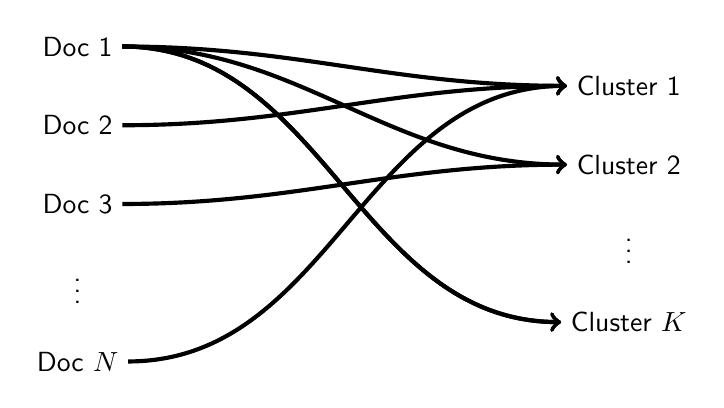
\begin{tikzpicture}

\node (doc1) at (-8,5.5) [] {Doc 1} ;
\node (doc2) at (-8, 4.5) [] {Doc 2} ;
\node (doc3) at (-8, 3.5) [] {Doc 3} ;
\node (doc4) at (-8, 2.5) [] {$\vdots$} ;
\node (doc5) at ( -8, 1.5) [] {Doc $N$} ;


\node (clust1) at (-1, 5) [] {Cluster 1} ;
\node (clust2) at (-1, 4) [] {Cluster 2} ;
\node (clustd) at (-1, 3) [] {$\vdots$} ;
\node (clust4) at (-1, 2) [] {Cluster $K$} ;

\invisible<1,3->{\draw[->, line width = 1.5pt]  (doc1)  to [out=0, in=180] (clust4) ; }
\invisible<1-2,4->{\draw[->, line width = 1.5pt]  (doc2)  to [out=0, in=180] (clust1) ; }
\invisible<1-3,5->{\draw[->, line width = 1.5pt]  (doc3)  to [out=0, in=180] (clust2) ; }
\invisible<1-4,6->{\draw[->, line width = 1.5pt]  (doc5)  to [out=0, in=180] (clust1) ; }

\invisible<1-6>{\draw[->, line width= 1.5pt] (doc1) to [out=0, in =180] (clust1) ;
\draw[->, line width= 1.5pt] (doc1) to [out=0, in =180] (clust2) ;
\draw[->, line width= 1.5pt] (doc1) to [out=0, in =180] (clust4) ;
}


\end{tikzpicture}

\pause \pause \pause \pause \pause \pause

\end{frame}


\begin{frame}
\frametitle{A Statistical Highlighter (With Many Colors) }


\scalebox{0.45}{\includegraphics{WallachHighlighter.png}}

\end{frame}



\begin{frame}
\frametitle{Vanilla Latent Dirichlet Allocation$\leadsto$ Objective Function}

\begin{itemize}
\item[-] Consider document $i$, $(i =1, 2, \hdots, N)$.
\invisible<1>{\item[-] Suppose there are $M_{i}$ total words and $\boldsymbol{x}_{i}$ is an $M_{i} \times 1$ vector, where $x_{im}$ describes the $m^{\text{th}}$ word used in the document$^{*}$.    }
\end{itemize}


\begin{eqnarray}
\invisible<1-6>{\boldsymbol{\theta}_{k} & \sim & \text{Dirichlet}(\boldsymbol{1}) \nonumber }\\
\invisible<1-7>{\alpha_{k} & \sim & \text{Gamma}(\alpha, \beta) \nonumber } \\
\invisible<1-3>{\boldsymbol{\pi}_{i}|\boldsymbol{\alpha} & \sim & \text{Dirichlet}(\boldsymbol{\alpha}) }\nonumber \\
\invisible<1-4>{\boldsymbol{\tau}_{im}| \boldsymbol{\pi}_{i} & \sim & \text{Multinomial}(1, \boldsymbol{\pi}_{i})} \nonumber \\
\invisible<1-5>{x_{im} | \boldsymbol{\theta}_{k}, \tau_{imk}=1 & \sim & \text{Multinomial}(1, \boldsymbol{\theta}_{k}) }\nonumber
\end{eqnarray}


\invisible<1-2, 4->{$^{*}$Notice: this is a different representation than a document-term matrix.  $x_{im}$ is a number that says which of the $J$ words are used.  The difference is for clarity and we'll this representation is closely related to document-term matrix}


\pause \pause \pause \pause \pause \pause \pause
\end{frame}


\begin{frame}
\frametitle{Vanilla Latent Dirichlet Allocation$\leadsto$ Objective Function}

Together the model implies the following posterior:

\begin{small}
\begin{eqnarray}
\invisible<1>{p(\boldsymbol{\pi}, \boldsymbol{T},\boldsymbol{\Theta}, \boldsymbol{\alpha}| \boldsymbol{X}) & \propto & \nonumber p(\boldsymbol{\alpha}) p(\boldsymbol{\pi}| \boldsymbol{\alpha}) p(\boldsymbol{T}| \boldsymbol{\pi}) p(\boldsymbol{X}| \boldsymbol{\theta}, \boldsymbol{T}) \nonumber } \\
\invisible<1-2>{& \propto & p(\boldsymbol{\alpha}) \prod_{i=1}^{N} \left[p(\boldsymbol{\pi}_{i} | \boldsymbol{\alpha}) \prod_{m=1}^{M_{i}} p(\boldsymbol{\tau}_{im}| \boldsymbol{\pi}) p(x_{im}| \boldsymbol{\theta}_{k}, \tau_{imk}=1) \right ] \nonumber }\\
\invisible<1-3>{& \propto & p(\boldsymbol{\alpha}) \prod_{i=1}^{N} \left[\alert<5>{\frac{\Gamma(\sum_{k=1}^{K} \alpha_{k})}{\prod_{k=1}^{K} \Gamma(\alpha_{k}) } \prod_{k=1}^{K} \pi_{ik}^{\alpha_{k}- 1}} \prod_{m=1}^{M}\prod_{k=1}^{K} \left[ \pi_{ik} \alert<6>{\prod_{j=1}^{J} \theta_{jk}^{x_{imj}} }  \right]^{\tau_{ikm}} \right] }\nonumber
\end{eqnarray}

\end{small}

\invisible<1-6>{Optimization:}
\begin{itemize}
\invisible<1-7>{\item[-] Variational Approximation$\leadsto$ Find ``closest" distribution}
\invisible<1-8>{\item[-] Gibbs sampling $\leadsto$ MCMC algorithm to approximate posterior}
\end{itemize}

\invisible<1-9>{\alert{Described in the slides appendix}}
\pause \pause \pause \pause \pause \pause \pause \pause \pause


\end{frame}


\begin{frame}
\frametitle{Why does this work$\leadsto$ Co-occurrence}


Where's the information for each word's topic? \pause \\

\invisible<1>{Reconsider document-term matrix} \pause

\begin{center}
\invisible<1-2>{\begin{tabular}{ccccc}
\hline
        & $\text{Word}_1$ & $\text{Word}_2$ & $\hdots$ & $\text{Word}_J$ \\
\hline
Doc$_{1}$  & 0   & 1    & $\hdots$ & 0 \\
Doc$_{2}$ & 2 & 0  & $\hdots$ & 3\\
$\vdots$ & $\vdots$ & $\vdots$ & $\ddots$ & $\vdots$ \\
Doc$_{N}$ & 0 & 1 & $\hdots$ & 1 \\
\hline\hline
\end{tabular}} \pause
\end{center}
\invisible<1-3>{Inner product of Documents (rows): $\textbf{Doc}_{i}^{'} \textbf{Doc}_{l} $} \pause \\
\vspace{0.1in}
\invisible<1-4>{Inner product of Terms (columns): $\textbf{Word}_j^{'} \textbf{Word}_k$ } \pause \\
\invisible<1-5>{\alert{Allows}: measure of correlation of term usage across documents (heuristically: partition words, based on usage in documents)} \pause \\
\invisible<1-6>{\alert{Latent Semantic Analysis}:  Reduce information in matrix using linear algebra (provides similar results, difficult to generalize)} \pause \\
\invisible<1-7>{\alert{Biclustering}: Models that partition documents and words simultaneously}

\end{frame}

\begin{frame}

{\tt R Code!}

\end{frame}





\begin{frame}
\frametitle{Types of Classification Problems}


\alert{Topic}: What is this text about? \pause
\invisible<1>{\begin{itemize}
\item[-] Policy area of legislation  \\
$\Rightarrow$ $\{$Agriculture, Crime, Environment, ...$\}$
\item[-] Campaign agendas \\
$\Rightarrow$ $\{$Abortion, Campaign, Finance, Taxing, ...       $\}$
\end{itemize}} \pause

\invisible<1-2>{\alert{Sentiment}: What is said in this text? [\alert{Public Opinion}] } \pause
\invisible<1-3>{\begin{itemize}
\item[-] Positions on legislation\\
 $\Rightarrow$ $\{$ Support, Ambiguous, Oppose $\}$
\item[-] Positions on Court Cases \\
$\Rightarrow$ $\{$ Agree with Court, Disagree with Court $\}$
\item[-] Liberal/Conservative Blog Posts \\
$\Rightarrow$ $\{$ Liberal, Middle, Conservative, No Ideology Expressed $\}$
\end{itemize} } \pause

\invisible<1-4>{\alert{Style}/\alert{Tone}: How is it said?} \pause
\invisible<1-5>{\begin{itemize}
\item[-] Taunting in floor statements\\
 $\Rightarrow$ $\{$ Partisan Taunt, Intra party taunt, Agency taunt, ... $\}$
\item[-] Negative campaigning \\
$\Rightarrow$ $\{$ Negative ad, Positive ad$\}$
\end{itemize} }

\end{frame}






\begin{frame}
\frametitle{Pre-existing word weights$\leadsto$ Dictionaries}

\invisible<1>{{\tt DICTION}}\\

\invisible<1>{\only<2>{\scalebox{0.55}{\includegraphics{DICTION2.png}}}}
\only<3>{\scalebox{0.55}{\includegraphics{DICTION3.png}}}
\only<4>{\scalebox{0.55}{\includegraphics{DICTION4.png}}}
\only<5>{\scalebox{0.85}{\includegraphics{DICTION5.png}}}
\only<6>{\scalebox{0.85}{\includegraphics{DictionCost.png}}}

\pause \pause \pause \pause \pause

\end{frame}


\begin{frame}

\scalebox{0.75}{\includegraphics{Year.jpg}}


\end{frame}

\begin{frame}
\frametitle{Dictionary Methods}


Many Dictionary Methods (like DICTION) \pause

\begin{itemize}
\invisible<1>{\item[1)] Proprietary}\pause\invisible<1-2>{$\leadsto$ wrapped in GUI} \pause
\invisible<1-3>{\item[2)] Basic tasks:} \pause
\begin{itemize}
\invisible<1-4>{\item[a)] Count words} \pause
\invisible<1-5>{\item[b)] Weighted counts of words} \pause
\invisible<1-6>{\item[c)] Some graphics}\pause
\end{itemize}
\invisible<1-7>{\item[3)] Pricey$\leadsto$ \alert{inexplicably}}
\end{itemize}



\end{frame}


\begin{frame}
\frametitle{DICTION}



\begin{columns}[]

\column{0.5\textwidth}
\scalebox{0.15}{\includegraphics{PolTone.jpg}}


\column{0.5\textwidth}
\pause
\begin{itemize}
\item[-] \invisible<1>{$\{$ Certain, Uncertain $\}$}\pause\invisible<1-2>{\\, $\{$ Optimistic, Pessimistic $\}$} \pause
\item[-] \invisible<1-3>{$\approx$ 10,000 words} \pause
\end{itemize}


\invisible<1-4>{Applies DICTION to a wide array of political texts\\} \pause
\invisible<1-5>{Examine specific periods of American political history}


\end{columns}



\end{frame}


\begin{frame}
\frametitle{Other Dictionaries }


\begin{itemize}
\item[1)] General Inquirer Database (\url{http://www.wjh.harvard.edu/~inquirer/} ) \pause
\begin{itemize}
\invisible<1>{\item[-] Stone, P.J., Dumphy, D.C., and Ogilvie, D.M. (1966) \emph{The General Inquirer: A Computer Approach to Content Analysis}} \pause
\invisible<1-2>{\item[-] $\{$ Positive, Negative $\}$ } \pause
\invisible<1-3>{\item[-] 3627 negative and positive word strings } \pause
\invisible<1-4>{\item[-] Workhorse for classification across many domains/papers} \pause
\end{itemize}
\invisible<1-5>{\item[2)] Linguistic Inquiry Word Count (LIWC)} \pause
\begin{itemize}
\invisible<1-6>{\item[-] Creation process:} \pause
\begin{itemize}
\invisible<1-7>{\item[1)] Generate word list for categories$\leadsto$ `` We drew on common emotion rating scales...Roget's Thesaurus...standard English dictionaries. [then] brain-storming sessions among 3-6 judges were held" to generate other words } \pause
\invisible<1-8>{\item[2)] Judge round$\leadsto$ (a) Does the word belong? (b) What other categories might it belong to?} \pause
\end{itemize}
\invisible<1-9>{\item[-] $\{$ Positive emotion, Negative emotion $\}$} \pause
\invisible<1-10>{\item[-] 2300 words grouped into 70 classes} \pause
\end{itemize}
\invisible<1-11>{\item[-] Harvard-IV-4 } \pause
\invisible<1-12>{\item[-] Affective Norms for English Words (we'll discuss this more later)} \pause
\invisible<1-13>{\item[-] ...}
\end{itemize}


\end{frame}





\begin{frame}
\frametitle{Generating New Words}

Three ways to create dictionaries (non-exhaustive): \pause
\begin{itemize}
\invisible<1>{\item[-] Statistical methods (Separating methods)} \pause
\invisible<1-2>{\item[-] Manual generation } \pause
\begin{itemize}
\invisible<1-3>{\item[-] Careful thought (prayer? epiphanies? divine intervention?) about useful words} \pause
\end{itemize}
\invisible<1-4>{\item[-] Populations of people who are surprisingly willing to perform ill-defined tasks} \pause
\begin{itemize}
\invisible<1-5>{\item[a)] Undergraduates$:\text{Pizza}\rightarrow \text{Research Output}$} \pause
\invisible<1-6>{\item[b)] Mechanical turkers} \pause
\begin{itemize}
\invisible<1-7>{\item[-] Example: $\{$ Happy, Unhappy $\}$ } \pause
\invisible<1-8>{\item[-] Ask turkers: how happy is } \pause
\invisible<1-9>{\item[] {\tt elevator}, {\tt car}, {\tt pretty}, {\tt young} } \pause
\invisible<1-10>{\item[] Output as dictionary}
\end{itemize}
\end{itemize}
\end{itemize}


\end{frame}





\begin{frame}
\frametitle{Applying Methods to Documents}

Applying the model: \pause
\begin{itemize}
\invisible<1>{\item[-] Vector of word counts:  $\boldsymbol{X}_i = (X_{i1}, X_{i2}, \hdots, X_{iK}$, $(i = 1, \hdots, N)$} \pause
\invisible<1-2>{\item[-] Weights attached to words  $\boldsymbol{\theta} = (\theta_{1}, \theta_{2}, \hdots, \theta_{K})$  } \pause
\begin{itemize}
\invisible<1-3>{\item[-] $\theta_{k} \in \{0,1\}$} \pause
\invisible<1-4>{\item[-] $\theta_{k} \in \{-1, 0, 1 \}$} \pause
\invisible<1-5>{\item[-] $\theta_{k} \in \{-2, -1, 0, 1, 2\}$} \pause
\invisible<1-6>{\item[-] $\theta_{k} \in \Re$} \pause
\end{itemize}
\end{itemize}

\invisible<1-7>{For each document $i$ calculate score for document } \pause
\begin{eqnarray}
\invisible<1-8>{Y_i  & = &  \frac{\sum_{k=1}^{K} \theta_k X_{ik}}{\sum_{k=1}^{K} X_{k}} \nonumber \\} \pause
\invisible<1-9>{Y_i  & = &  \frac{\boldsymbol{\theta}^{'} \boldsymbol{X}_i}{\boldsymbol{X}_{i}^{'} \boldsymbol{1} } \nonumber } \pause
\end{eqnarray}

\invisible<1-10>{$Y_{i} \approx $ continuous $\leadsto$ Classification} \pause
\begin{itemize}
\invisible<1-11>{\item[] $Y_i> 0 \Rightarrow$ Positive Category} \pause
\invisible<1-12>{\item[] $Y_i< 0 \Rightarrow$ Negative Category} \pause
\invisible<1-13>{\item[] $Y_i \approx 0$ Ambiguous}
\end{itemize}


\end{frame}


\begin{frame}
\frametitle{Applying a Dictionary to Press Releases}

\pause
\begin{itemize}
\invisible<1>{\item[-] Collection of 169,779 press releases (US House members 2005-2010)} \pause
\invisible<1-2>{\item[-] Dictionary from Neal Caren's website $\leadsto$ Theresa Wilson, Janyce Wiebe, and Paul Hoffman's dictionary } \pause
\invisible<1-3>{\item[-] Create positive/negative score for press releases.  }
\end{itemize}






\invisible<1-4>{{\tt Python} code and press releases}

\pause
\end{frame}


\begin{frame}
\frametitle{Examining Positive and Negative Statements in Press Releases}

\pause

\only<1-10>{
\invisible<1>{Least positive members of Congress:}
\begin{itemize}
\invisible<1-2>{\item[1)] Dan Burton, 2008}
\invisible<1-3>{\item[2)] Nancy Pelosi, 2007}
\invisible<1-4>{\item[3)] Mike Pence 2007}
\invisible<1-5>{\item[4)] John Boehner, 2009}
\invisible<1-6>{\item[5)] Jeff Flake, (basically all years)}
\invisible<1-7>{\item[6)] Eric Cantor, 2009}
\invisible<1-8>{\item[7)] Tom Price, 2010}
\end{itemize}

\invisible<1-9>{Legislators who are more extreme$\leadsto$ less positive in press releases}

}


\only<11>{\scalebox{0.5}{\includegraphics{pressOverTime.pdf}}}

\only<12-13>{
\begin{itemize}
\item[-] Credit Claiming press release: 9.1 percentage points ``more positive" than a non-credit claiming press release
\invisible<1-12>{\item[-] Anti-spending press release: 10.6 percentage points ``less positive" than a non-anti spending press release}
\end{itemize}
}

\only<14>{\scalebox{0.5}{\includegraphics{CreditPositive.pdf}}}
\only<15->{\scalebox{0.5}{\includegraphics{AntiCreditPositive.pdf}}}






\pause \pause \pause \pause \pause\pause \pause \pause \pause \pause \pause \pause \pause \pause


\end{frame}



\begin{frame}
\frametitle{Methodological Issues/Problems with Dictionaries}

\alert{Dictionary methods are context invariant} \pause \\
\begin{itemize}
\invisible<1>{\item[-] No optimization step $\leadsto$ same word weights regardless of texts} \pause
\invisible<1-2>{\item[-] Optimization$\leadsto$ incorporate information specific to context} \pause
\invisible<1-3>{\item[-] Without optimization$\leadsto$ unclear about dictionaries performance} \pause
\end{itemize}



\invisible<1-4>{\alert{Just because dictionaries provide measures labeled ``positive" or ``negative" it doesn't mean they are accurate measures in your text} (!!!!) \\} \pause

\vspace{0.5in}

\invisible<1-5>{{\huge \alert{Validation}}}


\end{frame}





\begin{frame}
\frametitle{Validation}

Classification Validity: \pause
\begin{itemize}
\invisible<1>{\item[-] \alert{Training}: build dictionary on subset of documents \alert{with known labels}} \pause
\invisible<1-2>{\item[-] \alert{Test}: apply dictionary method to other documents \alert{with known labels}} \pause
\invisible<1-3>{\item[-] Requires hand coded documents} \pause
\invisible<1-4>{\item[-] Hand coded documents useful for other reasons} \pause
\begin{itemize}
\invisible<1-5>{\item[-] Is the classification scheme well defined for your texts?} \pause
\invisible<1-6>{\item[-] Can humans accomplish the coding task?} \pause
\invisible<1-7>{\item[-] Is the dictionary your using appropriate?} \pause
\end{itemize}
\end{itemize}

\large
\invisible<1-8>{\alert{Replicate} classification exercise}  \pause
\normalsize
\begin{itemize}
\invisible<1-9>{\item[-] How well does our method perform on \alert{held out} documents?} \pause
\invisible<1-10>{\item[-] Why held out?} \pause \invisible<1-11>{\alert{Over fitting} } \pause
\invisible<1-12>{\item[-] Using off-the-shelf dictionary: all labeled documents to test} \pause
\invisible<1-13>{\item[-] Supervised learning classification: \alert{(Cross)validation} }
\end{itemize}

\end{frame}

\begin{frame}
\frametitle{Hand Coding: A Brief Digression}

\alert{Humans should be able to classify documents into the categories you want the machine to classify them in} \pause
\begin{itemize}
\invisible<1>{\item[-] This is \alert{hard}} \pause
\invisible<1-2>{\item[-] Why? } \pause
\begin{itemize}
\invisible<1-3>{\item[-] Ambiguity in language} \pause
\invisible<1-4>{\item[-] Limited working memory} \pause
\invisible<1-5>{\item[-] Ambiguity in classification rules} \pause
\end{itemize}
\invisible<1-6>{\item[-] A procedure for training coders: } \pause
\invisible<1-7>{\begin{itemize}
\item[1)] Coding rules
\item[2)] Apply to new texts
\item[3)] Assess coder agreement (we'll discuss more in a few weeks)
\item[4)] Using information and discussion, revise coding rules
\end{itemize}}
\end{itemize}
\end{frame}



\begin{frame}
\frametitle{Assessing Classification}

Measures of classification performance

\begin{tabular}{l|l|l}
 \hline
  & \multicolumn{2}{c}{Actual Label}  \\
  \hline
  Guess &   Liberal & Conservative \\
  \hline
  Liberal &  \alert{True Liberal} & False Liberal \\
  \hline
  Conservative & False Conservative & \alert{True Conservative} \\
  \hline
  \hline
\end{tabular}

\pause
\begin{eqnarray}
\invisible<1>{\text{Accuracy} & = & \frac{ \alert{\text{TrueLib} }+ \alert{\text{TrueCons}}  } { \alert{\text{TrueLib} } + \alert{\text{TrueCons}} + \text{FalseLib} + \text{FalseCons} } \nonumber } \pause  \\
\invisible<1-2>{\text{Precision}_{\text{Liberal}} &= &   \frac{ \alert{\text{True Liberal}}    }  { \alert{\text{True Liberal }} + \text{False Liberal}      } } \pause  \nonumber \\
\invisible<1-3>{\text{Recall}_{\text{Liberal} } & = & \frac{ \alert{\text{True Liberal}}   } { \alert{\text{True Liberal}} + \text{False Conservative}   } } \pause  \nonumber \\
\invisible<1-4>{F_{\text{Liberal}} & = & \frac{ 2\text{Precision}_{\text{Liberal}} \text{Recall}_{\text{Liberal} } } { \text{Precision}_{\text{Liberal}} +  \text{Recall}_{\text{Liberal} }} }   \nonumber \pause
\end{eqnarray}

\invisible<1-5>{\alert{Under reported for dictionary classification} }
\end{frame}


\begin{frame}
\frametitle{What about continuous measures?}

\pause

\invisible<1>{\alert{Necessarily more complicated}\\} \pause

\begin{itemize}
\invisible<1-2>{\item[-] Go back to hand coding exercise} \pause
\invisible<1-3>{\item[-] Imagine asking undergraduates to rate document on a continuous scale (0-100)} \pause
\invisible<1-4>{\item[-] \alert{Difficult} to create classifications with agreement} \pause
\invisible<1-5>{\item[-] \alert{Precisely} the point$\leadsto$ merely creating a gold standard is hard, let alone computer classification} \pause
\end{itemize}

\invisible<1-6>{\alert{Lower level classification}}\pause\invisible<1-7>{$\leadsto$ label phrases and then aggregate} \pause \\

\invisible<1-8>{Modifiable areal unit problem in texts}\pause$\leadsto$\invisible<1-9>{aggregating destroys information, conclusion may depend on level of aggregation}



\end{frame}







\begin{frame}
\frametitle{Validation, Dictionaries from other Fields}
\pause
\invisible<1>{Accounting Research: measure \alert{tone} of \alert{10-K} reports} \pause
\begin{itemize}
%\item[-] Comprehensive public summary of company performance
\invisible<1-2>{\item[-] \alert{tone} matters (\$)} \pause
\end{itemize}

\invisible<1-3>{Previous state of art: Harvard-IV-4 Dictionary applied to texts} \\
\invisible<1-4>{Loughran and McDonald (2011): \alert{Financial Documents are Different}, \textcolor{blue}{polysemes} } \pause
\begin{itemize}
\invisible<1-5>{\item[-] Negative words in Harvard, Not Negative in Accounting: \\} \pause
\invisible<1-6>{{\tt tax, cost, capital, board, liability, foreign,  cancer, crude (oil), tire } } \pause
\invisible<1-7>{\item[-] \alert{73\%} of Harvard negative words in this set(!!!!!)} \pause
\invisible<1-8>{\item[-] Not Negative Harvard, Negative in Accounting: \\} \pause
\invisible<1-9>{{\tt felony, litigation, restated, misstatement, and unanticipated} } \pause
\end{itemize}


\large
\invisible<1-10>{\alert{Context Matters}}


\end{frame}





\begin{frame}
\frametitle{Measuring Happiness}

\begin{columns}[]
\column{0.5\textwidth}
\scalebox{0.35}{\includegraphics{Bentham.jpg}}

\column{0.5\textwidth}

\pause
\begin{itemize}
\invisible<1>{\item[-] Quantifying Happiness: How happy is society?} \pause
\invisible<1-2>{\item[-] How Happy is a Song?} \pause
\invisible<1-3>{\item[-] Blog posts?} \pause
\invisible<1-4>{\item[-] Facebook posts? (Gross National Happiness)} \pause
\end{itemize}

\invisible<1-5>{Use \alert{Dictionary Methods} }

\end{columns}



\end{frame}


\begin{frame}
\frametitle{Measuring Happiness}

Dodds and Danforth (2009): Use a dictionary method to measure happiness \pause
\begin{itemize}
\invisible<1>{\item[-]  \alert{Affective Norms for English Words} (ANEW)} \pause
\invisible<1-2>{\item[-] Bradley and Lang 1999:  1034 words, Affective reaction to words} \pause
\begin{itemize}
\invisible<1-3>{\item[-] On a scale of 1-9 how happy does this word make you?} \pause
\invisible<1-4>{\item[] \alert{Happy} : triumphant (8.82)/paradise (8.72)/ love (8.72) } \pause
\invisible<1-5>{\item[] \alert{Neutral}: street (5.22)/ paper (5.20)/ engine (5.20) } \pause
\invisible<1-6>{\item[] \alert{Unhappy} : cancer (1.5)/funeral (1.39)/ rape (1.25) /suicide (1.25) } \pause
\end{itemize}
\invisible<1-7>{\item[-] \alert{Happiness} for text $i$ (with word $j$ having happiness $\theta_j$ and document frequence $X_{ij}$} \pause
\begin{eqnarray}
\invisible<1-8>{\text{Happiness}_{i}  & = & \frac{ \sum_{k=1}^{K} \theta_{k} X_{ik} } { \sum_{k=1}^{K} X_{ik}} }  \nonumber
\end{eqnarray}
\end{itemize}


\end{frame}



\begin{frame}



\scalebox{0.5}{\includegraphics{BillyJean.png}}
\pause


\invisible<1>{\alert{Homework Hints}:}
\invisible<1>{One approach: write a {\tt for} loop searching for words in dictionary (caution: is dictionary stemmed?) }\\ \pause
\invisible<1-2>{Happiest Song on Thriller?}  \\ \pause
\invisible<1-3>{\alert{P.Y.T. (Pretty Young Thing) }   (This is the right answer!)}


\end{frame}


\begin{frame}
\frametitle{Happiness in Society}

\only<1>{\scalebox{1}{\includegraphics{SongHappiness.png}}}
\only<2>{\scalebox{1}{\includegraphics{SongType.png}}}
\only<3>{\scalebox{0.7}{\includegraphics{Blog.png}}}

\end{frame}





\begin{frame}
\frametitle{Supervised Learning}

\invisible<1>{Supervised Methods: } \pause
\begin{itemize}
\invisible<1-2>{\item[-] Models for \alert{categorizing texts}} \pause
\begin{itemize}
\invisible<1-3>{\item[-] Know (develop) categories before hand} \pause
\invisible<1-4>{\item[-] Hand coding: assign documents to categories
\item[-] Infer: new document assignment to categories (distribution of documents to categories)} \pause
\invisible<1-5>{\item[-] \alert{Pre-estimation}: extensive work constructing categories, building classifiers
\item[-] \alert{Post-estimation}: relatively little work}
\end{itemize}
\end{itemize}


\end{frame}

\begin{frame}
\frametitle{Supervised Learning}

\pause
\begin{itemize}
\invisible<1>{\item[-] How to generate \alert{valid} hand coding categories} \pause
\begin{itemize}
\invisible<1-2>{\item[-] Assessing coder performance
\item[-] Assessing disagreement among coders
\item[-] Evidence coders perform well} \pause
\end{itemize}
\invisible<1-3>{\item[-] Supervised Learning Methods: \alert{Naive Bayes}, \alert{LASSO} (Ridge), \alert{ReadMe} } \pause
\invisible<1-4>{\item[-] Assessing Model Performance}  \pause
\end{itemize}


\invisible<1-5>{\alert{Methods generalize beyond text} }


\end{frame}


\begin{frame}
\frametitle{Components to Supervised Learning Method}


 \pause
\begin{itemize}
\invisible<1>{\item[1)] Set of \alert{categories}  } \pause
\begin{itemize}
\invisible<1-2>{\item[-] Credit Claiming, Position Taking, Advertising
\item[-] Positive Tone, Negative Tone
\item[-] Pro-war, Ambiguous, Anti-war} \pause
\end{itemize}
\invisible<1-3>{\item[2)] Set of \alert{hand-coded} documents } \pause
\begin{itemize}
\invisible<1-4>{\item[-] Coding done by human coders
\item[-] \alert{Training} Set: documents we'll use to learn how to code
\item[-] \alert{Validation} Set: documents we'll use to learn how well we code } \pause
\end{itemize}
\invisible<1-5>{\item[3)] Set of \alert{unlabeled} documents} \pause
\invisible<1-6>{\item[4)] Method to extrapolate from hand coding to unlabeled documents}
\end{itemize}


\end{frame}



\begin{frame}
\frametitle{How Do We Generate Coding Rules and Categories?}

\pause
\invisible<1>{\alert{Challenge}: coding rules/training coders to maximize coder performance} \pause \\
\invisible<1-2>{\alert{Challenge}: developing a clear set of categories} \pause
\begin{itemize}
\invisible<1-3>{\item[1)] Limits of Humans:} \pause
\begin{itemize}
\invisible<1-4>{\item[-] Small working memories
\item[-] Easily distracted
\item[-] Insufficient motivation} \pause
\end{itemize}
\invisible<1-5>{\item[2)] Limits of Language:} \pause
\begin{itemize}
\invisible<1-6>{\item[-] Fundamental ambiguity in language [careful analysis of texts]
\item[-] Contextual nature of language}
\end{itemize}
\end{itemize}

\pause

\invisible<1-7>{For supervised methods to work: maximize coder agreement (without cheating!)} \pause
\begin{itemize}
\invisible<1-8>{\item[1)] Write careful (and brief) coding rules } \pause
\begin{itemize}
\invisible<1-9>{\item[-] Flow charts help simplify problems } \pause
\end{itemize}
\invisible<1-10>{\item[2)] Train coders to remove ambiguity, misinterpretation}
\end{itemize}

\end{frame}


\begin{frame}
\frametitle{How Do We Generate Coding Rules?}

Iterative process for generating coding rules:\pause
\begin{itemize}
\invisible<1>{\item[1)] Write a set of coding rules} \pause
\invisible<1-2>{\item[2)] Have coders code documents (about 200) } \pause
\invisible<1-3>{\item[3)] Assess coder agreement } \pause
\invisible<1-4>{\item[4)] Identify sources of disagreement, repeat }
\end{itemize}



\end{frame}


\begin{frame}
\frametitle{How Do We Identify Coding Disagreement?}

\alert{Many} measures of inter-coder agreement\\
Essentially attempt to summarize a \alert{confusion} matrix\\

\begin{tabular}{l|l|l|l|l||l}
\hline
 & Cat 1& Cat 2 & Cat 3 & Cat 4  & Sum, Coder 1\\
 \hline
 Cat 1 &  \textbf{30}  & 0      &  \alert{1}          & 0         &       31             \\
 \hline
 Cat 2 & 1   &     \textbf{1}  &      0       &   0        &  2     \\
 \hline
 Cat 3&  0  &   0    &  \textbf{1}           &   0        & 1       \\
 \hline
 Cat 4  &  \alert{3}  &  1   &  0      &  \textbf{7}    &   11                \\
 \hline\hline
 Sum, Coder 2& 34   &  2     &  2          &   7        &     Total: \textbf{45}    \\
 \hline
\end{tabular}

\begin{itemize}
\item[-] \textbf{Diagonal}: coders agree on document
\item[-] \alert{Off-diagonal} : coders disagree (confused) on document
\end{itemize}


\alert{Generalize} across ($k$) coders:
\begin{itemize}
\item[-]  $\frac{k (k-1) }{2} $ pairwise comparisons
\item[-] $k$ comparisons: Coder A against All other coders
\end{itemize}

\end{frame}


\begin{frame}
\frametitle{How Do We Identify Coding Disagreements?}

During coding development phase/coder assessment phase, \alert{full} confusion matrices help to identify
\begin{itemize}
\item[-] Ambiguity
\item[-] Coder slacking
\end{itemize}
Example: 3 Coders, 8 categories.

\only<2>{\scalebox{0.5}{\includegraphics{Coder1.png}}}
\only<3>{\scalebox{0.5}{\includegraphics{Coder2.png}}}
\only<4>{\scalebox{0.5}{\includegraphics{Coder3.png}}}

\end{frame}



\begin{frame}
\frametitle{Example Coding Document}


8 part coding scheme
\begin{itemize}
\item[-] \alert{Across Party Taunting}: explicit public and negative attacks on the other party or its members
\item[-] \alert{Within Party Taunting}: explicit public and negative attacks on the same party or its members [for 1960's politics]
\item[-] \alert{Other taunting}: explicit public and negative attacks not directed at a party
\item[-] \alert{Bipartisan support}: praise for the other party
\item[-] \alert{Honorary Statements}: qualitatively different kind of speech
\item[-] \alert{Policy speech}: a speech without taunting or credit claiming
\item[-] \alert{Procedural}
\item[-] \alert{No Content}: (occasionally occurs in CR)
\end{itemize}


\end{frame}



\begin{frame}
\frametitle{Example Coding Document}



\scalebox{0.5}{\includegraphics{TauntingFig.png}}



\end{frame}



\begin{frame}
\frametitle{How Do We Summarize Confusion Matrix?}

Lots of statistics to summarize confusion matrix:
\begin{itemize}
\item[-] \alert{Most common}: intercoder agreement
\end{itemize}

\begin{eqnarray}
\text{Inter Coder}(A, B) & = & \frac{\text{No. (Coder A \& Coder B agree) }  } { \text{No. Documents}  } \nonumber
\end{eqnarray}


\end{frame}

\begin{frame}

\alert{Liberal} measure of agreement: \pause
\begin{itemize}
\invisible<1>{\item[-] Some agreement by \alert{chance}} \pause
\invisible<1-2>{\item[-] Consider coding scheme with two categories \\
 $\{$ Class 1, Class 2$\}$. } \pause
\invisible<1-3>{\item[-] Coder $A$ and Coder $B$ flip a (biased coin).   \\
$($ Pr(Class 1) = 0.75, Pr(Class 2) = 0.25 $)$ } \pause
\invisible<1-4>{\item[-] Inter Coder reliability: \alert{0.625 } } \pause
\end{itemize}

\invisible<1-5>{What to do?} \pause \\
\invisible<1-6>{Suggestion: \alert{Subtract off amount expected by chance:} } \pause
\begin{itemize}
\invisible<1-7>{\item[]$\text{Inter Coder} (A,B)_{\text{norm}}  =  $
\item[]$   \frac{\text{No. (Coder A \& Coder B agree)} - \text{No. Expected by Chance}  }   { \text{No. Documents}  }$  } \pause
\end{itemize}

\invisible<1-8>{\alert{Question}: what is amount expected by chance? } \pause
\begin{itemize}
\invisible<1-9>{\item[-] $\frac{1}{\# \text{Categories}}$ ?
\item[-] Avg Proportion in categories across coders?  (Krippendorf's Alpha)  } \pause
\end{itemize}

\invisible<1-10>{\alert{Best Practice}: present confusion matrices. } \\

\end{frame}

\begin{frame}
\frametitle{Krippendorf's Alpha}

Define coder reliability as: \pause
\begin{eqnarray}
\invisible<1>{\alpha & = & 1- \frac{\text{No. Pairwise Disagreements Observed }} {\text{No Pairwise Disagreements Expected By Chance}} \nonumber } \pause
\end{eqnarray}
\begin{itemize}
\invisible<1-2>{\item[] No. Pairwise Disagreements Observed = observe from data} \pause
\invisible<1-3>{\item[] No Expected pairwise disagreements: coding by chance, with rate labels used available from data } \pause
\end{itemize}

\invisible<1-4>{Thinking through expected differences: }\pause
\begin{itemize}
\invisible<1-5>{\item[-] Pretend I know something I'm trying to estimate
\item[-] How is that we know coders estimate levels well?
\item[-] Have to present correlation statistic: vary assumptions about ``expectations" (from uniform, to data driven)} \pause
\end{itemize}


\invisible<1-6>{Calculate in {\tt R} with {\tt concord} package and function {\tt kripp.alpha} }

\end{frame}



\begin{frame}
\frametitle{How Many To Code By Hand/How Many to Code By Machine}


Rules of thumb:
\begin{itemize}
\item[-] Hopkins and King (2010): \alert{500 documents} likely sufficient
\item[-] Hopkins and King (2010): \alert{100 documents} may be enough
\item[-] \alert{BUT}: depends on quantity of interest
\item[-] May \alert{REQUIRE} many more documents
\end{itemize}

\end{frame}

\begin{frame}
\frametitle{Percent data coded, Error (From Dan Jurafsky) }


\scalebox{0.35}{\includegraphics{TestError.png}}


\end{frame}




\begin{frame}
\frametitle{Three categories of documents}

\alert{Hand labeled}
\begin{itemize}
\item[-] Training set (what we'll use to estimate model)
\item[-] Validation set (what we'll use to assess model)
\end{itemize}
\alert{Unlabeled}
\begin{itemize}
\item[-] Test set (what we'll use the model to categorize)
\end{itemize}

\alert{Label more documents than necessary to train model}


\end{frame}



\begin{frame}
\frametitle{Regression models}

Suppose we have $N$ documents, with each document $i$ having label $y_{i} \in \{-1, 1\}\leadsto\{$liberal, conservative$\}$ \pause \\
\invisible<1>{We represent each document $i$ is $\boldsymbol{x}_{i} = (x_{i1}, x_{i2}, \hdots, x_{iJ})$. } \pause  \\

\begin{eqnarray}
\invisible<1-2>{f(\boldsymbol{\beta}, \boldsymbol{X}, \boldsymbol{Y})  & = & \sum_{i=1}^{N}\left( y_{i} - \boldsymbol{\beta}^{'} \boldsymbol{x}_{i} \right)^{2}  \nonumber \\} \pause
\invisible<1-3>{\widehat{\boldsymbol{\beta} } & = & \text{arg min}_{\boldsymbol{\beta}} \left\{\sum_{i=1}^{N}\left( y_{i} - \boldsymbol{\beta}^{'} \boldsymbol{x}_{i} \right)^{2}\right\} \nonumber \\} \pause
 \invisible<1-4>{& = & \left( \boldsymbol{X}^{'}\boldsymbol{X}   \right)^{-1}\boldsymbol{X}^{'}\boldsymbol{Y} \nonumber } \pause
\end{eqnarray}

\invisible<1-5>{Problem: \\} \pause
\begin{itemize}
\invisible<1-6>{\item[-] $J$ will likely be large (perhaps $J> N$)} \pause
\invisible<1-7>{\item[-] There many correlated variables} \pause
\end{itemize}

\invisible<1-8>{Predictions will be \alert{variable}}


\end{frame}



\begin{frame}
\frametitle{Lasso Regression Objective Function/Optimization}

Penalty for Model Complexity

\begin{eqnarray}
f(\boldsymbol{\beta}, \boldsymbol{X}, \boldsymbol{Y} ) & = & \sum_{i=1}^{N} \left(y_{i} - \beta_{0} + \sum_{j=1}^{J} \beta_{j} x_{ij}  \right)^{2} + \lambda \sum_{j=1}^{J} \underbrace{|\beta_{j}|}_{\text{Penalty}} \nonumber \pause
\end{eqnarray}


\begin{itemize}
\invisible<1>{\item[-] Optimization is non-linear (Absolute Value)} \pause
\begin{itemize}
\invisible<1-2>{\item[-] Coordinate Descent} \pause
\invisible<1-3>{\item[-] Start with Ridge} \pause
\invisible<1-4>{\item[-] Sub-differential, update steps} \pause
\end{itemize}
\invisible<1-5>{\item[-] Induces \alert{sparsity}$\leadsto$ sets some coefficients to zero}
\end{itemize}

\end{frame}



\begin{frame}
\frametitle{Selecting $\lambda$}

How do we determine $\lambda$? $\leadsto$ Cross validation  \pause \\
\invisible<1>{Applying models gives score (probability) of document belong to class$\leadsto$ threshold to classify} \pause \\

{\tt To the R code!}

\end{frame}



\begin{frame}
\frametitle{Assessing Models (Elements of Statistical Learning) }


\begin{itemize}
\item[-] \alert{Model Selection}: tuning parameters to select final model (next week's discussion)
\item[-] \alert{Model assessment}: after selecting model, estimating error in classification
\end{itemize}


\end{frame}


\begin{frame}
\frametitle{Comparing Training and Validation Set}

Text classification and model assessment
\begin{itemize}
\item[-] \alert{Replicate} classification exercise with \alert{validation} set
\item[-] General \alert{principle} of classification/prediction
\item[-] Compare supervised learning labels to hand labels
\end{itemize}

\alert{Confusion matrix}


\end{frame}



\begin{frame}
\frametitle{Comparing Training and Validation Set}

Representation of Test Statistics from Dictionary week (along with some new ones) \\


\begin{tabular}{l|l|l}
 \hline
  & \multicolumn{2}{c}{Actual Label}  \\
  \hline
  Classification (algorithm) &   Liberal & Conservative \\
  \hline
  Liberal &  \alert{True Liberal} & False Liberal \\
  \hline
  Conservative & False Conservative & \alert{True Conservative} \\
  \hline
  \hline
\end{tabular}

\pause
\begin{eqnarray}
\invisible<1>{\text{Accuracy} & = & \frac{ \alert{\text{TrueLib} }+ \alert{\text{TrueCons}}  } { \alert{\text{TrueLib} } + \alert{\text{TrueCons}} + \text{FalseLib} + \text{FalseCons} } \nonumber } \pause  \\
\invisible<1-2>{\text{Precision}_{\text{Liberal}} &= &   \frac{ \alert{\text{True Liberal}}    }  { \alert{\text{True Liberal }} + \text{False Liberal}      } } \pause  \nonumber \\
\invisible<1-3>{\text{Recall}_{\text{Liberal} } & = & \frac{ \alert{\text{True Liberal}}   } { \alert{\text{True Liberal}} + \text{False Conservative}   } } \pause  \nonumber \\
\invisible<1-4>{F_{\text{Liberal}} & = & \frac{ 2\text{Precision}_{\text{Liberal}} \text{Recall}_{\text{Liberal} } } { \text{Precision}_{\text{Liberal}} +  \text{Recall}_{\text{Liberal} }} }   \nonumber \pause
\end{eqnarray}

\end{frame}


% \begin{frame}
% \frametitle{Precision Recall Tradeoff}



% \scalebox{0.4}{\includegraphics{PrecRecall.pdf}}



% \end{frame}




\begin{frame}
\frametitle{ROC Curve}

ROC as a measure of model performance
\begin{eqnarray}
\text{Recall}_{\text{Liberal}} & = & \frac{\text{True Liberal}  } {\text{True Liberal} + \text{False Conservative}  }\nonumber \\
\text{Recall}_{\text{Conservative}} & =  & \frac{\text{True Conservative}  } {\text{True Conservative} + \text{False Liberal}  }\nonumber
\end{eqnarray}

\alert{Tension}:
\begin{itemize}
\item[-] Everything liberal: Recall$_{\text{Liberal}}$ =1 ; $\text{Recall}_{\text{Conservative}}=0$
\item[-] Everything conservative: Recall$_{\text{Liberal}}$ =0 ; $\text{Recall}_{\text{Conservative}}=1$
\end{itemize}

Characterize Tradeoff: \\
Plot True Positive Rate $\text{Recall}_{\text{Liberal}}$ \\
 False Positive Rate (1 - $\text{Recall}_{\text{Conservative}}$)



\end{frame}




\begin{frame}
\frametitle{Precision/Recall Tradeoff}

\scalebox{0.4}{\includegraphics{ROC.pdf}}


\end{frame}

\begin{frame}
\frametitle{Simple Classification Example}

Analyzing house press releases\\
\alert{Hand Code}: 1,000 press releases
\begin{itemize}
\item[-] Advertising
\item[-] Credit Claiming
\item[-] Position Taking
\end{itemize}
Divide 1,000 press releases into two sets
\begin{itemize}
\item[-] 500: Training set
\item[-] 500: Test set
\end{itemize}

\alert{Initial exploration}: provides baseline measurement at classifier performances \\
\alert{Improve}: through improving model fit
\end{frame}





\begin{frame}
\frametitle{Example from Grimmer, Westwood, and Messing (2014)}



\begin{tabular}{l|lll}
 & \multicolumn{3}{c}{Actual Label} \\
 \hline
Classification (Naive Bayes) & Position Taking & Advertising & Credit Claim. \\
Position Taking   &    10  &   0  &   0 \\
Advertising   & 2  & 40  &  2 \\
Credit Claiming   &   80 & 60 & 306\\
\hline\hline
\end{tabular}

\footnotesize
\begin{eqnarray}
\text{Accuracy} & = & \frac{10 + 40 + 306} {500}  = 0.71 \nonumber  \\
\text{Precision}_{PT} & = & \frac{10}{10}  = 1 \nonumber \\
\text{Recall}_{PT} & = & \frac{10}{10 + 2 + 80 }  = 0.11 \nonumber \\
\text{Precision}_{AD} & = & \frac{40}{40 + 2 + 2}  = 0.91 \nonumber \\
\text{Recall}_{AD} & = & \frac{40}{40 + 60 }  = 0.4 \nonumber \\
\text{Precision}_{Credit} & = & \frac{306}{306  + 80 + 60 } = 0.67 \nonumber  \\
\text{Recall}_{Credit} & = & \frac{306}{306 + 2}  = 0.99 \nonumber
\end{eqnarray}

\end{frame}



\begin{frame}
\frametitle{ReadMe: Optimization for a Different Goal (Hopkins and King 2010) }

Naive Bayes, LASSO, $\hdots$: focused on individual document classification. \pause \\
\invisible<1>{But what if we're focused on \alert{proportions only}? } \pause  \\
\invisible<1-2>{Hopkins and King (2010): method for characterizing distribution of classes} \pause  \\
\invisible<1-3>{\alert{Can be much more accurate than individual classifiers}, requires fewer assumptions (\alert{do not need random sample of documents } ) .} \pause
\begin{itemize}
\invisible<1-4>{\item[-] King and Lu (2008): derive method for characterizing causes of deaths for verbal autopsies }\pause
\invisible<1-5>{\item[-] Hopkins and King (2010): extend the method to text documents } \pause
\end{itemize}


\invisible<1-6>{Basic intuition: } \pause
\begin{itemize}
\invisible<1-7>{\item[-] Examine joint distribution of characteristics (without making Naive Bayes like assumption)
\item[-] Focus on distributions (only) makes this analysis possible}
\end{itemize}


\end{frame}



\begin{frame}
\frametitle{ReadMe: Optimization for a Different Goal (Hopkins and King 2010) }

Measure \alert{only} presence/absence of each term [$(J x 1) $ vector ] \pause
\begin{eqnarray}
\invisible<1>{\boldsymbol{x}_i & = & (1, 0, 0, 1, \hdots, 0) \nonumber } \pause
\end{eqnarray}

\invisible<1-2>{What are the possible realizations of $\boldsymbol{x}_i$?} \pause
\begin{itemize}
\invisible<1-3>{\item[-] $2^{J}$ possible vectors} \pause
\end{itemize}

\invisible<1-4>{Define:} \pause
\begin{eqnarray}
\invisible<1-5>{P(\boldsymbol{x}) & = & \text{probability of observing } \boldsymbol{x}} \pause  \nonumber \\
\invisible<1-6>{P(\boldsymbol{x}|C_j) & = & \text{Probability of observing } \boldsymbol{x} \text{ conditional on category } C_j} \pause  \nonumber \\
\invisible<1-7>{P(\boldsymbol{X}| C) & = & \text{Matrix collecting vectors} } \pause \nonumber \\
\invisible<1-8>{P(C ) & = & P(C_1, C_2, \hdots, C_K) \text{ target quantity of interest } } \pause \nonumber
\end{eqnarray}



\end{frame}



\begin{frame}
\frametitle{ReadMe: Optimization for a Different Goal (Hopkins and King 2010) }

\begin{eqnarray}
\underbrace{P(\boldsymbol{x} )}_{2^{J} x 1}  & = & \underbrace{P(\boldsymbol{x}| C )}_{2^{J} x K}  \underbrace{P(C)}_{K x 1 }  \nonumber
\end{eqnarray}
Matrix algebra problem to solve, for $P(C)$ \\
Like Naive Bayes, requires two pieces to estimate\\
Complication $2^{J} >> \text{no. documents} $\\
\alert{Kernel Smoothing Methods} (without a formal model)
\begin{itemize}
\item[-] $P(\boldsymbol{x})$ = estimate directly from test set
\item[-] $P(\boldsymbol{x}| C)$ = estimate from training set
\begin{itemize}
\item[-] Key assumption: $P(\boldsymbol{x}| C)$ in training set is equivalent to $P(\boldsymbol{x}| C)$ in test set
\end{itemize}
\item[-] If true, can perform biased sampling of documents, worry less about drift...
\end{itemize}


\end{frame}

\begin{frame}
\frametitle{Algorithm Summarized}

\begin{itemize}
\item[-] Estimate $\hat{p}(\boldsymbol{x})$ from test set
\item[-] Estimate $\hat{p}(\boldsymbol{x}|C)$ from training set
\item[-] Use $\hat{p}(\boldsymbol{x})$ and $\hat{p}(\boldsymbol{x}|C)$ to solve for $p(C)$
\end{itemize}


\end{frame}


\begin{frame}
\frametitle{Assessing Model Performance}

Not classifying individual documents $\rightarrow$ different standards\\
\alert{Mean Square Error} :
\begin{eqnarray}
\text{E}[(\hat{\theta} - \theta) ^2] & = & \text{var} (\hat{\theta} ) + \text{Bias}(\hat{\theta},  \theta)^2 \nonumber
\end{eqnarray}
Suppose we have true proportions $P(C)^{\text{true}}$.  Then, we'll estimate \alert{Root Mean Square Error }
\begin{eqnarray}
\text{RMSE} & = & \sqrt{ \frac{\sum_{j=1}^{J} (P(C_j)^{\text{true}} - P(C_j) ) } {J} } \nonumber \\
\text{Mean Abs. Prediction Error} & = & | \frac{\sum_{j=1}^{J} (P(C_j)^{\text{true}} - P(C_j) ) } {J} | \nonumber
\end{eqnarray}

\alert{Visualize}: plot true and estimated proportions


\end{frame}


\begin{frame}
\begin{center}
\only<1>{\scalebox{0.8}{\includegraphics{Shot1.png}}}
\end{center}
\only<2>{\scalebox{0.5}{\includegraphics{Shot2.png}}}

\end{frame}

\begin{frame}
\frametitle{Using the House Press Release Data}

\begin{tabular}{lll}
\hline\hline
Method & RMSE & APSE  \\
\hline
ReadMe &  0.036  & 0.056 \\
NaiveBayes & 0.096 & 0.14 \\
SVM & 0.052 & 0.084 \\
\hline
\end{tabular}


\end{frame}


\begin{frame}
\frametitle{Code to Run in R}


Control file: \\
\begin{tabular}{lll}
filename & truth & trainingset \\
\hline
20July2009LEWIS53.txt & 4 & \alert{1} \\
26July2006LEWIS249.txt & 2 & \alert{0} \\
\hline
\end{tabular}



{\tt tdm<- undergrad(control=control, fullfreq=F)  } \\
{\tt process<- preprocess(tdm) } \\
{\tt output<- undergrad(process) } \\
{\tt output\$est.CSMF \#\# proportion in each category} \\
{\tt output\$true.CSMF \#\# if labeled for validation set (but not used in training set) }



\end{frame}







\end{document}
